\documentclass[11pt]{ctexart}
% Shared preamble of the v4 papers (Chinese; xelatex with ctex).
\usepackage[margin=1in]{geometry}
\usepackage{amsmath,amssymb}
\usepackage{booktabs,multirow,array}
\usepackage{graphicx}
\usepackage[font=small,labelfont=bf]{caption}
\usepackage{subcaption}
\usepackage{xcolor}
\usepackage{enumitem}
\usepackage[numbers,sort&compress]{natbib}
\usepackage[hidelinks]{hyperref}
\usepackage{url}
\setlist{nosep,leftmargin=*}
\newcommand{\kev}{Kev-4B}
\newcommand{\pc}{P_{\mathrm{c}}}
\newcommand{\pg}{P_{\mathrm{g}}}
\newcommand{\ci}[2]{[#1,\,#2]}
\newenvironment{correction}{\begin{center}\begin{minipage}{0.95\linewidth}\small\setlength{\parskip}{3pt}\noindent\textbf{更正声明。}}{\end{minipage}\end{center}}

% \NUM{key}: a number computed by dcjev/analysis/paper_numbers.py and written to the paper's numbers.tex.
% A key that numbers.tex does not define prints as ??key?? and logs a warning, so a missing number cannot vanish.
\makeatletter
\newcommand{\NUM}[1]{\ifcsname num@#1\endcsname\csname num@#1\endcsname\else\textbf{??\detokenize{#1}??}\PackageWarning{numbers}{Undefined number #1}\fi}
\newcommand{\defnum}[2]{\expandafter\def\csname num@#1\endcsname{#2}}
\makeatother

% Generated by dcjev/analysis/paper_numbers.py -- do not edit.
\defnum{acc_base_aime24}{10.0}
\defnum{acc_base_aime25}{10.9}
\defnum{acc_base_amc}{50.6}
\defnum{acc_base_gsm}{87.9}
\defnum{acc_base_math}{76.5}
\defnum{acc_rlvr_aime24}{21.5}
\defnum{acc_rlvr_aime24_s1}{21.0}
\defnum{acc_rlvr_aime24_s2}{21.9}
\defnum{acc_rlvr_aime25}{17.8}
\defnum{acc_rlvr_aime25_s1}{18.8}
\defnum{acc_rlvr_aime25_s2}{16.9}
\defnum{acc_rlvr_amc}{61.7}
\defnum{acc_rlvr_amc_s1}{63.6}
\defnum{acc_rlvr_amc_s2}{59.8}
\defnum{acc_rlvr_gsm}{93.2}
\defnum{acc_rlvr_gsm_s1}{93.0}
\defnum{acc_rlvr_gsm_s2}{93.3}
\defnum{acc_rlvr_math}{82.9}
\defnum{acc_rlvr_math_s1}{82.8}
\defnum{acc_rlvr_math_s2}{83.0}
\defnum{acc_treekev_aime24}{26.4}
\defnum{acc_treekev_aime24_s1}{31.9}
\defnum{acc_treekev_aime24_s2}{20.8}
\defnum{acc_treekev_aime25}{20.0}
\defnum{acc_treekev_aime25_s1}{24.4}
\defnum{acc_treekev_aime25_s2}{15.6}
\defnum{acc_treekev_amc}{65.8}
\defnum{acc_treekev_amc_s1}{68.4}
\defnum{acc_treekev_amc_s2}{63.1}
\defnum{acc_treekev_gsm}{94.1}
\defnum{acc_treekev_gsm_s1}{94.7}
\defnum{acc_treekev_gsm_s2}{93.5}
\defnum{acc_treekev_math}{84.9}
\defnum{acc_treekev_math_s1}{87.2}
\defnum{acc_treekev_math_s2}{82.6}
\defnum{acc_treerand_aime24}{27.2}
\defnum{acc_treerand_aime24_s1}{21.0}
\defnum{acc_treerand_aime24_s2}{33.3}
\defnum{acc_treerand_aime25}{20.5}
\defnum{acc_treerand_aime25_s1}{16.2}
\defnum{acc_treerand_aime25_s2}{24.8}
\defnum{acc_treerand_amc}{67.0}
\defnum{acc_treerand_amc_s1}{63.4}
\defnum{acc_treerand_amc_s2}{70.5}
\defnum{acc_treerand_gsm}{93.1}
\defnum{acc_treerand_gsm_s1}{92.4}
\defnum{acc_treerand_gsm_s2}{93.8}
\defnum{acc_treerand_math}{84.5}
\defnum{acc_treerand_math_s1}{82.4}
\defnum{acc_treerand_math_s2}{86.6}
\defnum{accsd_base_aime24}{0.0}
\defnum{accsd_base_aime25}{0.4}
\defnum{accsd_base_amc}{1.8}
\defnum{accsd_base_gsm}{0.3}
\defnum{accsd_base_math}{0.1}
\defnum{accsd_rlvr_aime24}{0.6}
\defnum{accsd_rlvr_aime25}{1.3}
\defnum{accsd_rlvr_amc}{2.7}
\defnum{accsd_rlvr_gsm}{0.2}
\defnum{accsd_rlvr_math}{0.1}
\defnum{accsd_treekev_aime24}{7.8}
\defnum{accsd_treekev_aime25}{6.2}
\defnum{accsd_treekev_amc}{3.8}
\defnum{accsd_treekev_gsm}{0.9}
\defnum{accsd_treekev_math}{3.3}
\defnum{accsd_treerand_aime24}{8.7}
\defnum{accsd_treerand_aime25}{6.0}
\defnum{accsd_treerand_amc}{5.0}
\defnum{accsd_treerand_gsm}{1.0}
\defnum{accsd_treerand_math}{3.0}
\defnum{allright_rlvr}{46\%}
\defnum{allright_treekev}{48\%}
\defnum{allright_treerand}{48\%}
\defnum{allwrong_rlvr}{14\%}
\defnum{allwrong_treekev}{16\%}
\defnum{allwrong_treerand}{14\%}
\defnum{auc_128_artrack}{0.77}
\defnum{auc_128_kevcorrect}{0.70}
\defnum{auc_128_kevtrack}{0.76}
\defnum{auc_128_logprob}{0.67}
\defnum{auc_256_artrack}{0.79}
\defnum{auc_256_kevcorrect}{0.75}
\defnum{auc_256_kevtrack}{0.77}
\defnum{auc_256_logprob}{0.72}
\defnum{auc_512_artrack}{0.79}
\defnum{auc_512_kevcorrect}{0.77}
\defnum{auc_512_kevtrack}{0.77}
\defnum{auc_512_logprob}{0.73}
\defnum{aucw_128_artrack}{0.63}
\defnum{aucw_128_kevcorrect}{0.59}
\defnum{aucw_128_kevtrack}{0.61}
\defnum{aucw_128_logprob}{0.64}
\defnum{aucw_256_artrack}{0.64}
\defnum{aucw_256_kevcorrect}{0.59}
\defnum{aucw_256_kevtrack}{0.64}
\defnum{aucw_256_logprob}{0.66}
\defnum{aucw_512_artrack}{0.67}
\defnum{aucw_512_kevcorrect}{0.58}
\defnum{aucw_512_kevtrack}{0.65}
\defnum{aucw_512_logprob}{0.64}
\defnum{aucwhi_128_artrack}{0.65}
\defnum{aucwhi_128_kevcorrect}{0.62}
\defnum{aucwhi_128_kevtrack}{0.64}
\defnum{aucwhi_128_logprob}{0.66}
\defnum{aucwhi_256_artrack}{0.67}
\defnum{aucwhi_256_kevcorrect}{0.62}
\defnum{aucwhi_256_kevtrack}{0.67}
\defnum{aucwhi_256_logprob}{0.69}
\defnum{aucwhi_512_artrack}{0.71}
\defnum{aucwhi_512_kevcorrect}{0.63}
\defnum{aucwhi_512_kevtrack}{0.69}
\defnum{aucwhi_512_logprob}{0.68}
\defnum{aucwlo_128_artrack}{0.60}
\defnum{aucwlo_128_kevcorrect}{0.57}
\defnum{aucwlo_128_kevtrack}{0.58}
\defnum{aucwlo_128_logprob}{0.61}
\defnum{aucwlo_256_artrack}{0.61}
\defnum{aucwlo_256_kevcorrect}{0.56}
\defnum{aucwlo_256_kevtrack}{0.61}
\defnum{aucwlo_256_logprob}{0.63}
\defnum{aucwlo_512_artrack}{0.63}
\defnum{aucwlo_512_kevcorrect}{0.54}
\defnum{aucwlo_512_kevtrack}{0.60}
\defnum{aucwlo_512_logprob}{0.59}
\defnum{auditbest_all_treekev}{$+$8.1}
\defnum{auditbest_all_treekev_s1}{$+$7.8}
\defnum{auditbest_all_treekev_s2}{$+$8.5}
\defnum{auditbest_all_treerand}{$+$8.1}
\defnum{auditbest_all_treerand_s1}{$+$8.3}
\defnum{auditbest_all_treerand_s2}{$+$8.0}
\defnum{auditbest_first20_treekev}{$+$12.3}
\defnum{auditbest_first20_treerand}{$+$16.1}
\defnum{auditbest_firsthalf_treekev}{$+$9.5}
\defnum{auditbest_firsthalf_treerand}{$+$9.4}
\defnum{auditbest_last20_treekev}{$+$6.2}
\defnum{auditbest_last20_treerand}{$+$7.5}
\defnum{auditbest_records_treekev}{40}
\defnum{auditbest_records_treerand}{40}
\defnum{auditbest_secondhalf_treekev}{$+$6.8}
\defnum{auditbest_secondhalf_treerand}{$+$6.9}
\defnum{auditgain_all_treekev}{$+$1.4}
\defnum{auditgain_all_treekev_s1}{$+$1.2}
\defnum{auditgain_all_treekev_s2}{$+$1.6}
\defnum{auditgain_all_treerand}{$+$0.2}
\defnum{auditgain_all_treerand_s1}{$+$0.7}
\defnum{auditgain_all_treerand_s2}{$-$0.2}
\defnum{auditgain_first20_treekev}{$+$4.9}
\defnum{auditgain_first20_treerand}{$+$2.1}
\defnum{auditgain_firsthalf_treekev}{$+$2.2}
\defnum{auditgain_firsthalf_treerand}{$+$0.6}
\defnum{auditgain_last20_treekev}{$+$0.9}
\defnum{auditgain_last20_treerand}{$-$0.9}
\defnum{auditgain_records_treekev}{40}
\defnum{auditgain_records_treerand}{40}
\defnum{auditgain_secondhalf_treekev}{$+$0.5}
\defnum{auditgain_secondhalf_treerand}{$-$0.1}
\defnum{auditgainhi_all_treekev}{2.1}
\defnum{auditgainhi_all_treerand}{0.8}
\defnum{auditgainlo_all_treekev}{0.7}
\defnum{auditgainlo_all_treerand}{$-$0.3}
\defnum{auditotauc_all_treekev}{0.75}
\defnum{auditotauc_all_treekev_s1}{0.74}
\defnum{auditotauc_all_treekev_s2}{0.77}
\defnum{auditotauc_all_treerand}{0.76}
\defnum{auditotauc_all_treerand_s1}{0.76}
\defnum{auditotauc_all_treerand_s2}{0.77}
\defnum{auditotauc_first20_treekev}{0.77}
\defnum{auditotauc_first20_treerand}{0.71}
\defnum{auditotauc_firsthalf_treekev}{0.75}
\defnum{auditotauc_firsthalf_treerand}{0.75}
\defnum{auditotauc_last20_treekev}{0.76}
\defnum{auditotauc_last20_treerand}{0.80}
\defnum{auditotauc_records_treekev}{40}
\defnum{auditotauc_records_treerand}{40}
\defnum{auditotauc_secondhalf_treekev}{0.76}
\defnum{auditotauc_secondhalf_treerand}{0.78}
\defnum{auditotaucw_all_treekev}{0.56}
\defnum{auditotaucw_all_treekev_s1}{0.56}
\defnum{auditotaucw_all_treekev_s2}{0.56}
\defnum{auditotaucw_all_treerand}{0.57}
\defnum{auditotaucw_all_treerand_s1}{0.57}
\defnum{auditotaucw_all_treerand_s2}{0.57}
\defnum{auditotaucw_first20_treekev}{0.65}
\defnum{auditotaucw_first20_treerand}{0.59}
\defnum{auditotaucw_firsthalf_treekev}{0.58}
\defnum{auditotaucw_firsthalf_treerand}{0.56}
\defnum{auditotaucw_last20_treekev}{0.52}
\defnum{auditotaucw_last20_treerand}{0.62}
\defnum{auditotaucw_records_treekev}{40}
\defnum{auditotaucw_records_treerand}{40}
\defnum{auditotaucw_secondhalf_treekev}{0.54}
\defnum{auditotaucw_secondhalf_treerand}{0.58}
\defnum{auditotaucwhi_all_treekev}{0.58}
\defnum{auditotaucwhi_all_treerand}{0.59}
\defnum{auditotaucwlo_all_treekev}{0.54}
\defnum{auditotaucwlo_all_treerand}{0.54}
\defnum{auditval_all_treekev}{59.5}
\defnum{auditval_all_treekev_s1}{59.1}
\defnum{auditval_all_treekev_s2}{59.9}
\defnum{auditval_all_treerand}{60.8}
\defnum{auditval_all_treerand_s1}{58.5}
\defnum{auditval_all_treerand_s2}{63.1}
\defnum{auditval_first20_treekev}{45.1}
\defnum{auditval_first20_treerand}{47.0}
\defnum{auditval_firsthalf_treekev}{53.0}
\defnum{auditval_firsthalf_treerand}{55.4}
\defnum{auditval_last20_treekev}{73.1}
\defnum{auditval_last20_treerand}{73.1}
\defnum{auditval_records_treekev}{40}
\defnum{auditval_records_treerand}{40}
\defnum{auditval_secondhalf_treekev}{66.0}
\defnum{auditval_secondhalf_treerand}{66.1}
\defnum{d_treekev_aime24}{$+$4.9}
\defnum{d_treekev_aime25}{$+$2.2}
\defnum{d_treekev_amc}{$+$4.1}
\defnum{d_treekev_gsm}{$+$0.9}
\defnum{d_treekev_math}{$+$2.0}
\defnum{d_treerand_aime24}{$+$5.7}
\defnum{d_treerand_aime25}{$+$2.7}
\defnum{d_treerand_amc}{$+$5.2}
\defnum{d_treerand_gsm}{$-$0.1}
\defnum{d_treerand_math}{$+$1.6}
\defnum{dhi_treekev_aime24}{10.0}
\defnum{dhi_treekev_aime25}{5.5}
\defnum{dhi_treekev_amc}{7.7}
\defnum{dhi_treekev_gsm}{1.7}
\defnum{dhi_treekev_math}{4.0}
\defnum{dhi_treerand_aime24}{10.3}
\defnum{dhi_treerand_aime25}{5.7}
\defnum{dhi_treerand_amc}{9.3}
\defnum{dhi_treerand_gsm}{0.8}
\defnum{dhi_treerand_math}{3.6}
\defnum{dlo_treekev_aime24}{0.3}
\defnum{dlo_treekev_aime25}{$-$0.7}
\defnum{dlo_treekev_amc}{0.7}
\defnum{dlo_treekev_gsm}{0.2}
\defnum{dlo_treekev_math}{0.1}
\defnum{dlo_treerand_aime24}{1.5}
\defnum{dlo_treerand_aime25}{$-$0.1}
\defnum{dlo_treerand_amc}{1.6}
\defnum{dlo_treerand_gsm}{$-$0.9}
\defnum{dlo_treerand_math}{$-$0.3}
\defnum{dvtreerand_rlvr_aime24}{$-$5.7}
\defnum{dvtreerand_rlvr_aime25}{$-$2.7}
\defnum{dvtreerand_rlvr_amc}{$-$5.2}
\defnum{dvtreerand_rlvr_gsm}{$+$0.1}
\defnum{dvtreerand_rlvr_math}{$-$1.6}
\defnum{dvtreerand_treekev_aime24}{$-$0.8}
\defnum{dvtreerand_treekev_aime25}{$-$0.5}
\defnum{dvtreerand_treekev_amc}{$-$1.2}
\defnum{dvtreerand_treekev_gsm}{$+$1.0}
\defnum{dvtreerand_treekev_math}{$+$0.4}
\defnum{dvtreerandhi_rlvr_aime24}{$-$1.5}
\defnum{dvtreerandhi_rlvr_aime25}{0.1}
\defnum{dvtreerandhi_rlvr_amc}{$-$1.6}
\defnum{dvtreerandhi_rlvr_gsm}{0.9}
\defnum{dvtreerandhi_rlvr_math}{0.3}
\defnum{dvtreerandhi_treekev_aime24}{1.6}
\defnum{dvtreerandhi_treekev_aime25}{2.6}
\defnum{dvtreerandhi_treekev_amc}{1.0}
\defnum{dvtreerandhi_treekev_gsm}{1.9}
\defnum{dvtreerandhi_treekev_math}{2.3}
\defnum{dvtreerandlo_rlvr_aime24}{$-$10.3}
\defnum{dvtreerandlo_rlvr_aime25}{$-$5.7}
\defnum{dvtreerandlo_rlvr_amc}{$-$9.3}
\defnum{dvtreerandlo_rlvr_gsm}{$-$0.8}
\defnum{dvtreerandlo_rlvr_math}{$-$3.6}
\defnum{dvtreerandlo_treekev_aime24}{$-$3.5}
\defnum{dvtreerandlo_treekev_aime25}{$-$3.5}
\defnum{dvtreerandlo_treekev_amc}{$-$3.4}
\defnum{dvtreerandlo_treekev_gsm}{0.2}
\defnum{dvtreerandlo_treekev_math}{$-$1.6}
\defnum{gain_128_artrack}{$+$0.045}
\defnum{gain_128_kevcorrect}{$+$0.040}
\defnum{gain_128_kevtrack}{$+$0.046}
\defnum{gain_128_logprob}{$+$0.052}
\defnum{gain_128_oracle}{$+$0.048}
\defnum{gain_256_artrack}{$+$0.069}
\defnum{gain_256_kevcorrect}{$+$0.043}
\defnum{gain_256_kevtrack}{$+$0.064}
\defnum{gain_256_logprob}{$+$0.065}
\defnum{gain_256_oracle}{$+$0.098}
\defnum{gain_512_artrack}{$+$0.048}
\defnum{gain_512_kevcorrect}{$+$0.021}
\defnum{gain_512_kevtrack}{$+$0.040}
\defnum{gain_512_logprob}{$+$0.040}
\defnum{gain_512_oracle}{$+$0.059}
\defnum{gainhi_128_artrack}{0.057}
\defnum{gainhi_128_kevcorrect}{0.052}
\defnum{gainhi_128_kevtrack}{0.058}
\defnum{gainhi_128_logprob}{0.063}
\defnum{gainhi_128_oracle}{0.063}
\defnum{gainhi_256_artrack}{0.085}
\defnum{gainhi_256_kevcorrect}{0.060}
\defnum{gainhi_256_kevtrack}{0.082}
\defnum{gainhi_256_logprob}{0.083}
\defnum{gainhi_256_oracle}{0.117}
\defnum{gainhi_512_artrack}{0.075}
\defnum{gainhi_512_kevcorrect}{0.046}
\defnum{gainhi_512_kevtrack}{0.067}
\defnum{gainhi_512_logprob}{0.067}
\defnum{gainhi_512_oracle}{0.086}
\defnum{gainlo_128_artrack}{0.033}
\defnum{gainlo_128_kevcorrect}{0.028}
\defnum{gainlo_128_kevtrack}{0.034}
\defnum{gainlo_128_logprob}{0.041}
\defnum{gainlo_128_oracle}{0.033}
\defnum{gainlo_256_artrack}{0.053}
\defnum{gainlo_256_kevcorrect}{0.026}
\defnum{gainlo_256_kevtrack}{0.047}
\defnum{gainlo_256_logprob}{0.048}
\defnum{gainlo_256_oracle}{0.080}
\defnum{gainlo_512_artrack}{0.022}
\defnum{gainlo_512_kevcorrect}{$-$0.003}
\defnum{gainlo_512_kevtrack}{0.015}
\defnum{gainlo_512_logprob}{0.014}
\defnum{gainlo_512_oracle}{0.034}
\defnum{gainpt_128_artrack}{$+$4.5}
\defnum{gainpt_128_kevcorrect}{$+$4.0}
\defnum{gainpt_128_kevtrack}{$+$4.6}
\defnum{gainpt_128_logprob}{$+$5.2}
\defnum{gainpt_256_artrack}{$+$6.9}
\defnum{gainpt_256_kevcorrect}{$+$4.3}
\defnum{gainpt_256_kevtrack}{$+$6.4}
\defnum{gainpt_256_logprob}{$+$6.5}
\defnum{gainpt_512_artrack}{$+$4.8}
\defnum{gainpt_512_kevcorrect}{$+$2.1}
\defnum{gainpt_512_kevtrack}{$+$4.0}
\defnum{gainpt_512_logprob}{$+$4.0}
\defnum{gainpthi_128_artrack}{5.7}
\defnum{gainpthi_128_kevcorrect}{5.2}
\defnum{gainpthi_128_kevtrack}{5.8}
\defnum{gainpthi_128_logprob}{6.3}
\defnum{gainpthi_256_artrack}{8.5}
\defnum{gainpthi_256_kevcorrect}{6.0}
\defnum{gainpthi_256_kevtrack}{8.2}
\defnum{gainpthi_256_logprob}{8.3}
\defnum{gainpthi_512_artrack}{7.5}
\defnum{gainpthi_512_kevcorrect}{4.6}
\defnum{gainpthi_512_kevtrack}{6.7}
\defnum{gainpthi_512_logprob}{6.7}
\defnum{gainptlo_128_artrack}{3.3}
\defnum{gainptlo_128_kevcorrect}{2.8}
\defnum{gainptlo_128_kevtrack}{3.4}
\defnum{gainptlo_128_logprob}{4.1}
\defnum{gainptlo_256_artrack}{5.3}
\defnum{gainptlo_256_kevcorrect}{2.6}
\defnum{gainptlo_256_kevtrack}{4.7}
\defnum{gainptlo_256_logprob}{4.8}
\defnum{gainptlo_512_artrack}{2.2}
\defnum{gainptlo_512_kevcorrect}{$-$0.3}
\defnum{gainptlo_512_kevtrack}{1.5}
\defnum{gainptlo_512_logprob}{1.4}
\defnum{gentok_rlvr}{76.0}
\defnum{gentok_treekev}{82.0}
\defnum{gentok_treerand}{63.0}
\defnum{kevauc_rlvr}{0.88}
\defnum{kevauc_treekev}{0.89}
\defnum{kevauc_treerand}{0.87}
\defnum{kevauctr_all_rlvr}{0.92}
\defnum{kevauctr_all_rlvr_s1}{0.91}
\defnum{kevauctr_all_rlvr_s2}{0.92}
\defnum{kevauctr_all_treekev}{0.92}
\defnum{kevauctr_all_treekev_s1}{0.91}
\defnum{kevauctr_all_treekev_s2}{0.92}
\defnum{kevauctr_all_treerand}{0.91}
\defnum{kevauctr_all_treerand_s1}{0.90}
\defnum{kevauctr_all_treerand_s2}{0.92}
\defnum{kevauctr_first20_rlvr}{0.90}
\defnum{kevauctr_first20_treekev}{0.89}
\defnum{kevauctr_first20_treerand}{0.88}
\defnum{kevauctr_firsthalf_rlvr}{0.92}
\defnum{kevauctr_firsthalf_treekev}{0.91}
\defnum{kevauctr_firsthalf_treerand}{0.91}
\defnum{kevauctr_last20_rlvr}{0.89}
\defnum{kevauctr_last20_treekev}{0.90}
\defnum{kevauctr_last20_treerand}{0.90}
\defnum{kevauctr_records_rlvr}{400}
\defnum{kevauctr_records_treekev}{400}
\defnum{kevauctr_records_treerand}{400}
\defnum{kevauctr_secondhalf_rlvr}{0.92}
\defnum{kevauctr_secondhalf_treekev}{0.92}
\defnum{kevauctr_secondhalf_treerand}{0.91}
\defnum{kevaucwtr_all_rlvr}{0.81}
\defnum{kevaucwtr_all_rlvr_s1}{0.82}
\defnum{kevaucwtr_all_rlvr_s2}{0.80}
\defnum{kevaucwtr_all_treekev}{0.80}
\defnum{kevaucwtr_all_treekev_s1}{0.81}
\defnum{kevaucwtr_all_treekev_s2}{0.79}
\defnum{kevaucwtr_all_treerand}{0.79}
\defnum{kevaucwtr_all_treerand_s1}{0.78}
\defnum{kevaucwtr_all_treerand_s2}{0.81}
\defnum{kevaucwtr_first20_rlvr}{0.82}
\defnum{kevaucwtr_first20_treekev}{0.74}
\defnum{kevaucwtr_first20_treerand}{0.77}
\defnum{kevaucwtr_firsthalf_rlvr}{0.82}
\defnum{kevaucwtr_firsthalf_treekev}{0.80}
\defnum{kevaucwtr_firsthalf_treerand}{0.80}
\defnum{kevaucwtr_last20_rlvr}{0.76}
\defnum{kevaucwtr_last20_treekev}{0.80}
\defnum{kevaucwtr_last20_treerand}{0.83}
\defnum{kevaucwtr_records_rlvr}{395}
\defnum{kevaucwtr_records_treekev}{395}
\defnum{kevaucwtr_records_treerand}{396}
\defnum{kevaucwtr_secondhalf_rlvr}{0.79}
\defnum{kevaucwtr_secondhalf_treekev}{0.80}
\defnum{kevaucwtr_secondhalf_treerand}{0.79}
\defnum{kevc_rlvr}{0.73}
\defnum{kevc_treekev}{0.76}
\defnum{kevc_treerand}{0.74}
\defnum{kevm_rlvr}{0.80}
\defnum{kevm_treekev}{0.84}
\defnum{kevm_treerand}{0.81}
\defnum{lecabs_gsm8k500}{0.6}
\defnum{lecabs_math500}{1.6}
\defnum{lecabs_val}{2.2}
\defnum{lecmax_gsm8k500}{1.0}
\defnum{lecmax_math500}{4.4}
\defnum{lecmax_val}{6.6}
\defnum{lecmean_gsm8k500}{$+$0.3}
\defnum{lecmean_math500}{$+$1.6}
\defnum{lecmean_val}{$+$0.9}
\defnum{lecruns_gsm8k500}{6}
\defnum{lecruns_math500}{6}
\defnum{lecruns_val}{6}
\defnum{len_rlvr}{594}
\defnum{len_treekev}{705}
\defnum{len_treerand}{556}
\defnum{lpdiff_rlvr}{0.005}
\defnum{lpdiff_treekev}{0.006}
\defnum{lpdiff_treerand}{0.007}
\defnum{otauc_all_treekev}{0.78}
\defnum{otauc_all_treekev_s1}{0.78}
\defnum{otauc_all_treekev_s2}{0.78}
\defnum{otauc_all_treerand}{0.75}
\defnum{otauc_all_treerand_s1}{0.76}
\defnum{otauc_all_treerand_s2}{0.74}
\defnum{otauc_first20_treekev}{0.77}
\defnum{otauc_first20_treerand}{0.76}
\defnum{otauc_firsthalf_treekev}{0.79}
\defnum{otauc_firsthalf_treerand}{0.77}
\defnum{otauc_last20_treekev}{0.78}
\defnum{otauc_last20_treerand}{0.73}
\defnum{otauc_records_treekev}{400}
\defnum{otauc_records_treerand}{400}
\defnum{otauc_secondhalf_treekev}{0.77}
\defnum{otauc_secondhalf_treerand}{0.73}
\defnum{otaucw_all_treekev}{0.52}
\defnum{otaucw_all_treekev_s1}{0.53}
\defnum{otaucw_all_treekev_s2}{0.52}
\defnum{otaucw_all_treerand}{0.53}
\defnum{otaucw_all_treerand_s1}{0.52}
\defnum{otaucw_all_treerand_s2}{0.53}
\defnum{otaucw_first20_treekev}{0.54}
\defnum{otaucw_first20_treerand}{0.58}
\defnum{otaucw_firsthalf_treekev}{0.51}
\defnum{otaucw_firsthalf_treerand}{0.54}
\defnum{otaucw_last20_treekev}{0.54}
\defnum{otaucw_last20_treerand}{0.51}
\defnum{otaucw_records_treekev}{400}
\defnum{otaucw_records_treerand}{399}
\defnum{otaucw_secondhalf_treekev}{0.53}
\defnum{otaucw_secondhalf_treerand}{0.51}
\defnum{ps_contacc}{37.8\%}
\defnum{ps_continuations}{18{,}060}
\defnum{ps_dead_128}{41\%}
\defnum{ps_dead_256}{47\%}
\defnum{ps_dead_512}{61\%}
\defnum{ps_prefixes}{4{,}515}
\defnum{ps_prefixes_128}{1889}
\defnum{ps_prefixes_256}{1593}
\defnum{ps_prefixes_512}{1033}
\defnum{ps_problems}{500}
\defnum{ps_selproblems_128}{401}
\defnum{ps_selproblems_256}{253}
\defnum{ps_selproblems_512}{93}
\defnum{ps_value_128}{0.41}
\defnum{ps_value_256}{0.39}
\defnum{ps_value_512}{0.29}
\defnum{ps_valueall_128}{0.39}
\defnum{ps_valueall_256}{0.32}
\defnum{ps_valueall_512}{0.16}
\defnum{ps_valueallpct_128}{38.6}
\defnum{ps_valueallpct_256}{32.4}
\defnum{ps_valueallpct_512}{16.5}
\defnum{psd_128_artracklogprob}{$+$0.099}
\defnum{psd_128_kevtrackartrack}{$-$0.011}
\defnum{psd_128_kevtracklogprob}{$+$0.088}
\defnum{psd_256_artracklogprob}{$+$0.073}
\defnum{psd_256_kevtrackartrack}{$-$0.020}
\defnum{psd_256_kevtracklogprob}{$+$0.053}
\defnum{psd_512_artracklogprob}{$+$0.057}
\defnum{psd_512_kevtrackartrack}{$-$0.020}
\defnum{psd_512_kevtracklogprob}{$+$0.037}
\defnum{psdhi_128_artracklogprob}{0.125}
\defnum{psdhi_128_kevtrackartrack}{0.006}
\defnum{psdhi_128_kevtracklogprob}{0.117}
\defnum{psdhi_256_artracklogprob}{0.097}
\defnum{psdhi_256_kevtrackartrack}{$-$0.004}
\defnum{psdhi_256_kevtracklogprob}{0.080}
\defnum{psdhi_512_artracklogprob}{0.087}
\defnum{psdhi_512_kevtrackartrack}{0.001}
\defnum{psdhi_512_kevtracklogprob}{0.071}
\defnum{psdlo_128_artracklogprob}{0.073}
\defnum{psdlo_128_kevtrackartrack}{$-$0.028}
\defnum{psdlo_128_kevtracklogprob}{0.061}
\defnum{psdlo_256_artracklogprob}{0.048}
\defnum{psdlo_256_kevtrackartrack}{$-$0.037}
\defnum{psdlo_256_kevtracklogprob}{0.026}
\defnum{psdlo_512_artracklogprob}{0.028}
\defnum{psdlo_512_kevtrackartrack}{$-$0.041}
\defnum{psdlo_512_kevtracklogprob}{0.003}
\defnum{psdw_128_artracklogprob}{$-$0.013}
\defnum{psdw_128_kevtrackartrack}{$-$0.016}
\defnum{psdw_128_kevtracklogprob}{$-$0.029}
\defnum{psdw_256_artracklogprob}{$-$0.014}
\defnum{psdw_256_kevtrackartrack}{$-$0.007}
\defnum{psdw_256_kevtracklogprob}{$-$0.021}
\defnum{psdw_512_artracklogprob}{$+$0.037}
\defnum{psdw_512_kevtrackartrack}{$-$0.027}
\defnum{psdw_512_kevtracklogprob}{$+$0.010}
\defnum{psdwhi_128_artracklogprob}{0.015}
\defnum{psdwhi_128_kevtrackartrack}{0.006}
\defnum{psdwhi_128_kevtracklogprob}{0.002}
\defnum{psdwhi_256_artracklogprob}{0.019}
\defnum{psdwhi_256_kevtrackartrack}{0.020}
\defnum{psdwhi_256_kevtracklogprob}{0.014}
\defnum{psdwhi_512_artracklogprob}{0.085}
\defnum{psdwhi_512_kevtrackartrack}{0.012}
\defnum{psdwhi_512_kevtracklogprob}{0.064}
\defnum{psdwlo_128_artracklogprob}{$-$0.041}
\defnum{psdwlo_128_kevtrackartrack}{$-$0.038}
\defnum{psdwlo_128_kevtracklogprob}{$-$0.061}
\defnum{psdwlo_256_artracklogprob}{$-$0.048}
\defnum{psdwlo_256_kevtrackartrack}{$-$0.033}
\defnum{psdwlo_256_kevtracklogprob}{$-$0.055}
\defnum{psdwlo_512_artracklogprob}{$-$0.010}
\defnum{psdwlo_512_kevtrackartrack}{$-$0.065}
\defnum{psdwlo_512_kevtracklogprob}{$-$0.042}
\defnum{rho_128_artrack}{0.55}
\defnum{rho_128_kevcorrect}{0.40}
\defnum{rho_128_kevtrack}{0.53}
\defnum{rho_128_logprob}{0.34}
\defnum{rho_256_artrack}{0.56}
\defnum{rho_256_kevcorrect}{0.48}
\defnum{rho_256_kevtrack}{0.52}
\defnum{rho_256_logprob}{0.42}
\defnum{rho_512_artrack}{0.50}
\defnum{rho_512_kevcorrect}{0.47}
\defnum{rho_512_kevtrack}{0.46}
\defnum{rho_512_logprob}{0.39}
\defnum{roansrep_treekev_s1_0}{3\%}
\defnum{roansrep_treekev_s1_100}{0\%}
\defnum{roansrep_treekev_s1_125}{0\%}
\defnum{roansrep_treekev_s1_150}{0\%}
\defnum{roansrep_treekev_s1_175}{0\%}
\defnum{roansrep_treekev_s1_25}{1\%}
\defnum{roansrep_treekev_s1_50}{0\%}
\defnum{roansrep_treekev_s1_75}{0\%}
\defnum{roansrep_treekev_s2_0}{4\%}
\defnum{roansrep_treekev_s2_100}{41\%}
\defnum{roansrep_treekev_s2_125}{60\%}
\defnum{roansrep_treekev_s2_150}{65\%}
\defnum{roansrep_treekev_s2_175}{59\%}
\defnum{roansrep_treekev_s2_25}{7\%}
\defnum{roansrep_treekev_s2_50}{11\%}
\defnum{roansrep_treekev_s2_75}{42\%}
\defnum{roansrep_treerand_s1_0}{3\%}
\defnum{roansrep_treerand_s1_100}{0\%}
\defnum{roansrep_treerand_s1_125}{0\%}
\defnum{roansrep_treerand_s1_150}{0\%}
\defnum{roansrep_treerand_s1_175}{0\%}
\defnum{roansrep_treerand_s1_25}{2\%}
\defnum{roansrep_treerand_s1_50}{1\%}
\defnum{roansrep_treerand_s1_75}{0\%}
\defnum{roansrep_treerand_s2_0}{6\%}
\defnum{roansrep_treerand_s2_100}{7\%}
\defnum{roansrep_treerand_s2_125}{1\%}
\defnum{roansrep_treerand_s2_150}{0\%}
\defnum{roansrep_treerand_s2_175}{0\%}
\defnum{roansrep_treerand_s2_25}{10\%}
\defnum{roansrep_treerand_s2_50}{2\%}
\defnum{roansrep_treerand_s2_75}{1\%}
\defnum{roansrepmax_treekev_s1}{0\%}
\defnum{roansrepmax_treekev_s2}{65\%}
\defnum{roansrepmax_treerand_s1}{1\%}
\defnum{roansrepmax_treerand_s2}{7\%}
\defnum{roboxmany_treekev_s1_0}{17\%}
\defnum{roboxmany_treekev_s1_100}{5\%}
\defnum{roboxmany_treekev_s1_125}{4\%}
\defnum{roboxmany_treekev_s1_150}{4\%}
\defnum{roboxmany_treekev_s1_175}{5\%}
\defnum{roboxmany_treekev_s1_25}{9\%}
\defnum{roboxmany_treekev_s1_50}{5\%}
\defnum{roboxmany_treekev_s1_75}{5\%}
\defnum{roboxmany_treekev_s2_0}{20\%}
\defnum{roboxmany_treekev_s2_100}{38\%}
\defnum{roboxmany_treekev_s2_125}{53\%}
\defnum{roboxmany_treekev_s2_150}{54\%}
\defnum{roboxmany_treekev_s2_175}{54\%}
\defnum{roboxmany_treekev_s2_25}{19\%}
\defnum{roboxmany_treekev_s2_50}{19\%}
\defnum{roboxmany_treekev_s2_75}{40\%}
\defnum{roboxmany_treerand_s1_0}{17\%}
\defnum{roboxmany_treerand_s1_100}{5\%}
\defnum{roboxmany_treerand_s1_125}{3\%}
\defnum{roboxmany_treerand_s1_150}{2\%}
\defnum{roboxmany_treerand_s1_175}{3\%}
\defnum{roboxmany_treerand_s1_25}{10\%}
\defnum{roboxmany_treerand_s1_50}{9\%}
\defnum{roboxmany_treerand_s1_75}{6\%}
\defnum{roboxmany_treerand_s2_0}{22\%}
\defnum{roboxmany_treerand_s2_100}{21\%}
\defnum{roboxmany_treerand_s2_125}{28\%}
\defnum{roboxmany_treerand_s2_150}{22\%}
\defnum{roboxmany_treerand_s2_175}{25\%}
\defnum{roboxmany_treerand_s2_25}{16\%}
\defnum{roboxmany_treerand_s2_50}{11\%}
\defnum{roboxmany_treerand_s2_75}{9\%}
\defnum{roonset_treekev_s1}{--}
\defnum{roonset_treekev_s2}{75}
\defnum{roonset_treerand_s1}{--}
\defnum{roonset_treerand_s2}{--}
\defnum{rootsdone_all_treekev}{1.3\%}
\defnum{rootsdone_all_treekev_s1}{1.5\%}
\defnum{rootsdone_all_treekev_s2}{1.1\%}
\defnum{rootsdone_all_treerand}{1.8\%}
\defnum{rootsdone_all_treerand_s1}{0.6\%}
\defnum{rootsdone_all_treerand_s2}{3.0\%}
\defnum{rootsdone_first20_treekev}{4.3\%}
\defnum{rootsdone_first20_treerand}{4.6\%}
\defnum{rootsdone_firsthalf_treekev}{1.7\%}
\defnum{rootsdone_firsthalf_treerand}{1.2\%}
\defnum{rootsdone_last20_treekev}{1.1\%}
\defnum{rootsdone_last20_treerand}{4.2\%}
\defnum{rootsdone_records_treekev}{400}
\defnum{rootsdone_records_treerand}{400}
\defnum{rootsdone_secondhalf_treekev}{0.9\%}
\defnum{rootsdone_secondhalf_treerand}{2.4\%}
\defnum{rorep_treekev_s1_0}{0.8\%}
\defnum{rorep_treekev_s1_100}{0.5\%}
\defnum{rorep_treekev_s1_125}{0.4\%}
\defnum{rorep_treekev_s1_150}{0.5\%}
\defnum{rorep_treekev_s1_175}{0.2\%}
\defnum{rorep_treekev_s1_25}{0.8\%}
\defnum{rorep_treekev_s1_50}{0.6\%}
\defnum{rorep_treekev_s1_75}{0.6\%}
\defnum{rorep_treekev_s2_0}{1.0\%}
\defnum{rorep_treekev_s2_100}{6.0\%}
\defnum{rorep_treekev_s2_125}{8.3\%}
\defnum{rorep_treekev_s2_150}{10.1\%}
\defnum{rorep_treekev_s2_175}{10.1\%}
\defnum{rorep_treekev_s2_25}{1.5\%}
\defnum{rorep_treekev_s2_50}{1.9\%}
\defnum{rorep_treekev_s2_75}{6.2\%}
\defnum{rorep_treerand_s1_0}{0.9\%}
\defnum{rorep_treerand_s1_100}{0.5\%}
\defnum{rorep_treerand_s1_125}{0.7\%}
\defnum{rorep_treerand_s1_150}{0.6\%}
\defnum{rorep_treerand_s1_175}{0.7\%}
\defnum{rorep_treerand_s1_25}{1.0\%}
\defnum{rorep_treerand_s1_50}{0.8\%}
\defnum{rorep_treerand_s1_75}{0.6\%}
\defnum{rorep_treerand_s2_0}{1.5\%}
\defnum{rorep_treerand_s2_100}{1.5\%}
\defnum{rorep_treerand_s2_125}{0.2\%}
\defnum{rorep_treerand_s2_150}{0.1\%}
\defnum{rorep_treerand_s2_175}{0.0\%}
\defnum{rorep_treerand_s2_25}{1.8\%}
\defnum{rorep_treerand_s2_50}{1.0\%}
\defnum{rorep_treerand_s2_75}{0.8\%}
\defnum{roright_treekev_s1_0}{53\%}
\defnum{roright_treekev_s1_100}{69\%}
\defnum{roright_treekev_s1_125}{67\%}
\defnum{roright_treekev_s1_150}{67\%}
\defnum{roright_treekev_s1_175}{72\%}
\defnum{roright_treekev_s1_25}{58\%}
\defnum{roright_treekev_s1_50}{65\%}
\defnum{roright_treekev_s1_75}{62\%}
\defnum{roright_treekev_s2_0}{49\%}
\defnum{roright_treekev_s2_100}{64\%}
\defnum{roright_treekev_s2_125}{66\%}
\defnum{roright_treekev_s2_150}{66\%}
\defnum{roright_treekev_s2_175}{63\%}
\defnum{roright_treekev_s2_25}{57\%}
\defnum{roright_treekev_s2_50}{63\%}
\defnum{roright_treekev_s2_75}{63\%}
\defnum{roright_treerand_s1_0}{50\%}
\defnum{roright_treerand_s1_100}{68\%}
\defnum{roright_treerand_s1_125}{65\%}
\defnum{roright_treerand_s1_150}{66\%}
\defnum{roright_treerand_s1_175}{66\%}
\defnum{roright_treerand_s1_25}{58\%}
\defnum{roright_treerand_s1_50}{64\%}
\defnum{roright_treerand_s1_75}{61\%}
\defnum{roright_treerand_s2_0}{48\%}
\defnum{roright_treerand_s2_100}{65\%}
\defnum{roright_treerand_s2_125}{68\%}
\defnum{roright_treerand_s2_150}{70\%}
\defnum{roright_treerand_s2_175}{70\%}
\defnum{roright_treerand_s2_25}{59\%}
\defnum{roright_treerand_s2_50}{63\%}
\defnum{roright_treerand_s2_75}{64\%}
\defnum{rotok_treekev_s1_0}{624}
\defnum{rotok_treekev_s1_100}{533}
\defnum{rotok_treekev_s1_125}{528}
\defnum{rotok_treekev_s1_150}{550}
\defnum{rotok_treekev_s1_175}{553}
\defnum{rotok_treekev_s1_25}{656}
\defnum{rotok_treekev_s1_50}{608}
\defnum{rotok_treekev_s1_75}{622}
\defnum{rotok_treekev_s2_0}{620}
\defnum{rotok_treekev_s2_100}{811}
\defnum{rotok_treekev_s2_125}{863}
\defnum{rotok_treekev_s2_150}{880}
\defnum{rotok_treekev_s2_175}{859}
\defnum{rotok_treekev_s2_25}{675}
\defnum{rotok_treekev_s2_50}{668}
\defnum{rotok_treekev_s2_75}{817}
\defnum{rotok_treerand_s1_0}{591}
\defnum{rotok_treerand_s1_100}{582}
\defnum{rotok_treerand_s1_125}{610}
\defnum{rotok_treerand_s1_150}{592}
\defnum{rotok_treerand_s1_175}{586}
\defnum{rotok_treerand_s1_25}{671}
\defnum{rotok_treerand_s1_50}{633}
\defnum{rotok_treerand_s1_75}{627}
\defnum{rotok_treerand_s2_0}{637}
\defnum{rotok_treerand_s2_100}{651}
\defnum{rotok_treerand_s2_125}{602}
\defnum{rotok_treerand_s2_150}{510}
\defnum{rotok_treerand_s2_175}{527}
\defnum{rotok_treerand_s2_25}{707}
\defnum{rotok_treerand_s2_50}{654}
\defnum{rotok_treerand_s2_75}{640}
\defnum{rotrunc_treekev_s1_0}{26\%}
\defnum{rotrunc_treekev_s1_100}{16\%}
\defnum{rotrunc_treekev_s1_125}{16\%}
\defnum{rotrunc_treekev_s1_150}{18\%}
\defnum{rotrunc_treekev_s1_175}{21\%}
\defnum{rotrunc_treekev_s1_25}{29\%}
\defnum{rotrunc_treekev_s1_50}{24\%}
\defnum{rotrunc_treekev_s1_75}{23\%}
\defnum{rotrunc_treekev_s2_0}{26\%}
\defnum{rotrunc_treekev_s2_100}{44\%}
\defnum{rotrunc_treekev_s2_125}{50\%}
\defnum{rotrunc_treekev_s2_150}{52\%}
\defnum{rotrunc_treekev_s2_175}{51\%}
\defnum{rotrunc_treekev_s2_25}{31\%}
\defnum{rotrunc_treekev_s2_50}{28\%}
\defnum{rotrunc_treekev_s2_75}{46\%}
\defnum{rotrunc_treerand_s1_0}{23\%}
\defnum{rotrunc_treerand_s1_100}{17\%}
\defnum{rotrunc_treerand_s1_125}{20\%}
\defnum{rotrunc_treerand_s1_150}{16\%}
\defnum{rotrunc_treerand_s1_175}{16\%}
\defnum{rotrunc_treerand_s1_25}{30\%}
\defnum{rotrunc_treerand_s1_50}{25\%}
\defnum{rotrunc_treerand_s1_75}{20\%}
\defnum{rotrunc_treerand_s2_0}{28\%}
\defnum{rotrunc_treerand_s2_100}{27\%}
\defnum{rotrunc_treerand_s2_125}{28\%}
\defnum{rotrunc_treerand_s2_150}{20\%}
\defnum{rotrunc_treerand_s2_175}{22\%}
\defnum{rotrunc_treerand_s2_25}{33\%}
\defnum{rotrunc_treerand_s2_50}{26\%}
\defnum{rotrunc_treerand_s2_75}{24\%}
\defnum{rptabs_math500}{0.7}
\defnum{rptmax_math500}{1.4}
\defnum{rptmean_math500}{$-$0.4}
\defnum{rptruns_math500}{6}
\defnum{sansrep_rlvr}{0\%}
\defnum{sansrep_rlvr_s1}{0\%}
\defnum{sansrep_rlvr_s2}{0\%}
\defnum{sansrep_treekev}{45\%}
\defnum{sansrep_treekev_s1}{0\%}
\defnum{sansrep_treekev_s2}{90\%}
\defnum{sansrep_treerand}{0\%}
\defnum{sansrep_treerand_s1}{0\%}
\defnum{sansrep_treerand_s2}{0\%}
\defnum{sboxmany_rlvr}{4\%}
\defnum{sboxmany_rlvr_s1}{2\%}
\defnum{sboxmany_rlvr_s2}{6\%}
\defnum{sboxmany_treekev}{56\%}
\defnum{sboxmany_treekev_s1}{18\%}
\defnum{sboxmany_treekev_s2}{94\%}
\defnum{sboxmany_treerand}{25\%}
\defnum{sboxmany_treerand_s1}{3\%}
\defnum{sboxmany_treerand_s2}{46\%}
\defnum{sboxnone_rlvr}{2.9\%}
\defnum{sboxnone_treekev}{4.8\%}
\defnum{sboxnone_treerand}{4.5\%}
\defnum{seeds_rlvr}{2}
\defnum{seeds_treekev}{2}
\defnum{seeds_treerand}{2}
\defnum{skevright_rlvr}{0.84}
\defnum{skevright_treekev}{0.89}
\defnum{skevright_treerand}{0.86}
\defnum{skevwrong_rlvr}{0.59}
\defnum{skevwrong_treekev}{0.61}
\defnum{skevwrong_treerand}{0.58}
\defnum{sps_rlvr}{120}
\defnum{sps_treekev}{97}
\defnum{sps_treerand}{95}
\defnum{srep_rlvr}{0.9\%}
\defnum{srep_rlvr_s1}{0.7\%}
\defnum{srep_rlvr_s2}{1.1\%}
\defnum{srep_treekev}{12.4\%}
\defnum{srep_treekev_s1}{0.5\%}
\defnum{srep_treekev_s2}{24.4\%}
\defnum{srep_treerand}{0.4\%}
\defnum{srep_treerand_s1}{0.6\%}
\defnum{srep_treerand_s2}{0.2\%}
\defnum{st100acc_rlvr_math}{83.2}
\defnum{st100acc_rlvr_math_s1}{84.0}
\defnum{st100acc_rlvr_math_s2}{82.4}
\defnum{st100acc_treekev_math}{82.4}
\defnum{st100acc_treekev_math_s1}{82.8}
\defnum{st100acc_treekev_math_s2}{82.0}
\defnum{st100acc_treerand_math}{80.5}
\defnum{st100acc_treerand_math_s1}{80.6}
\defnum{st100acc_treerand_math_s2}{80.4}
\defnum{st100accsd_rlvr_math}{1.1}
\defnum{st100accsd_treekev_math}{0.6}
\defnum{st100accsd_treerand_math}{0.1}
\defnum{st100allright_rlvr}{42\%}
\defnum{st100allright_treekev}{42\%}
\defnum{st100allright_treerand}{42\%}
\defnum{st100allwrong_rlvr}{19\%}
\defnum{st100allwrong_treekev}{22\%}
\defnum{st100allwrong_treerand}{19\%}
\defnum{st100auditbest_all_treekev}{$+$9.5}
\defnum{st100auditbest_all_treekev_s1}{$+$8.4}
\defnum{st100auditbest_all_treekev_s2}{$+$10.6}
\defnum{st100auditbest_all_treerand}{$+$9.4}
\defnum{st100auditbest_all_treerand_s1}{$+$9.6}
\defnum{st100auditbest_all_treerand_s2}{$+$9.3}
\defnum{st100auditbest_first20_treekev}{$+$12.3}
\defnum{st100auditbest_first20_treerand}{$+$16.1}
\defnum{st100auditbest_firsthalf_treekev}{$+$11.5}
\defnum{st100auditbest_firsthalf_treerand}{$+$11.7}
\defnum{st100auditbest_last20_treekev}{$+$8.3}
\defnum{st100auditbest_last20_treerand}{$+$9.1}
\defnum{st100auditbest_records_treekev}{20}
\defnum{st100auditbest_records_treerand}{20}
\defnum{st100auditbest_secondhalf_treekev}{$+$7.5}
\defnum{st100auditbest_secondhalf_treerand}{$+$7.2}
\defnum{st100auditgain_all_treekev}{$+$2.2}
\defnum{st100auditgain_all_treekev_s1}{$+$1.8}
\defnum{st100auditgain_all_treekev_s2}{$+$2.6}
\defnum{st100auditgain_all_treerand}{$+$0.6}
\defnum{st100auditgain_all_treerand_s1}{$+$1.5}
\defnum{st100auditgain_all_treerand_s2}{$-$0.4}
\defnum{st100auditgain_first20_treekev}{$+$4.9}
\defnum{st100auditgain_first20_treerand}{$+$2.1}
\defnum{st100auditgain_firsthalf_treekev}{$+$2.8}
\defnum{st100auditgain_firsthalf_treerand}{$+$1.1}
\defnum{st100auditgain_last20_treekev}{$+$0.7}
\defnum{st100auditgain_last20_treerand}{$+$0.7}
\defnum{st100auditgain_records_treekev}{20}
\defnum{st100auditgain_records_treerand}{20}
\defnum{st100auditgain_secondhalf_treekev}{$+$1.7}
\defnum{st100auditgain_secondhalf_treerand}{$+$0.1}
\defnum{st100auditgainhi_all_treekev}{3.4}
\defnum{st100auditgainhi_all_treerand}{1.4}
\defnum{st100auditgainlo_all_treekev}{1.1}
\defnum{st100auditgainlo_all_treerand}{$-$0.3}
\defnum{st100auditotauc_all_treekev}{0.75}
\defnum{st100auditotauc_all_treekev_s1}{0.73}
\defnum{st100auditotauc_all_treekev_s2}{0.77}
\defnum{st100auditotauc_all_treerand}{0.75}
\defnum{st100auditotauc_all_treerand_s1}{0.74}
\defnum{st100auditotauc_all_treerand_s2}{0.75}
\defnum{st100auditotauc_first20_treekev}{0.77}
\defnum{st100auditotauc_first20_treerand}{0.71}
\defnum{st100auditotauc_firsthalf_treekev}{0.74}
\defnum{st100auditotauc_firsthalf_treerand}{0.73}
\defnum{st100auditotauc_last20_treekev}{0.73}
\defnum{st100auditotauc_last20_treerand}{0.71}
\defnum{st100auditotauc_records_treekev}{20}
\defnum{st100auditotauc_records_treerand}{20}
\defnum{st100auditotauc_secondhalf_treekev}{0.76}
\defnum{st100auditotauc_secondhalf_treerand}{0.77}
\defnum{st100auditotaucw_all_treekev}{0.58}
\defnum{st100auditotaucw_all_treekev_s1}{0.57}
\defnum{st100auditotaucw_all_treekev_s2}{0.58}
\defnum{st100auditotaucw_all_treerand}{0.56}
\defnum{st100auditotaucw_all_treerand_s1}{0.54}
\defnum{st100auditotaucw_all_treerand_s2}{0.57}
\defnum{st100auditotaucw_first20_treekev}{0.65}
\defnum{st100auditotaucw_first20_treerand}{0.59}
\defnum{st100auditotaucw_firsthalf_treekev}{0.60}
\defnum{st100auditotaucw_firsthalf_treerand}{0.56}
\defnum{st100auditotaucw_last20_treekev}{0.55}
\defnum{st100auditotaucw_last20_treerand}{0.53}
\defnum{st100auditotaucw_records_treekev}{20}
\defnum{st100auditotaucw_records_treerand}{20}
\defnum{st100auditotaucw_secondhalf_treekev}{0.55}
\defnum{st100auditotaucw_secondhalf_treerand}{0.55}
\defnum{st100auditotaucwhi_all_treekev}{0.61}
\defnum{st100auditotaucwhi_all_treerand}{0.59}
\defnum{st100auditotaucwlo_all_treekev}{0.55}
\defnum{st100auditotaucwlo_all_treerand}{0.52}
\defnum{st100auditval_all_treekev}{53.0}
\defnum{st100auditval_all_treekev_s1}{49.8}
\defnum{st100auditval_all_treekev_s2}{56.2}
\defnum{st100auditval_all_treerand}{55.4}
\defnum{st100auditval_all_treerand_s1}{51.8}
\defnum{st100auditval_all_treerand_s2}{59.1}
\defnum{st100auditval_first20_treekev}{45.1}
\defnum{st100auditval_first20_treerand}{47.0}
\defnum{st100auditval_firsthalf_treekev}{42.3}
\defnum{st100auditval_firsthalf_treerand}{46.5}
\defnum{st100auditval_last20_treekev}{61.4}
\defnum{st100auditval_last20_treerand}{60.1}
\defnum{st100auditval_records_treekev}{20}
\defnum{st100auditval_records_treerand}{20}
\defnum{st100auditval_secondhalf_treekev}{63.7}
\defnum{st100auditval_secondhalf_treerand}{64.4}
\defnum{st100d_treekev_math}{$-$0.8}
\defnum{st100d_treerand_math}{$-$2.7}
\defnum{st100dhi_treekev_math}{1.3}
\defnum{st100dhi_treerand_math}{$-$0.6}
\defnum{st100dlo_treekev_math}{$-$2.9}
\defnum{st100dlo_treerand_math}{$-$4.9}
\defnum{st100dvtreerand_rlvr_math}{$+$2.7}
\defnum{st100dvtreerand_treekev_math}{$+$1.9}
\defnum{st100dvtreerandhi_rlvr_math}{4.9}
\defnum{st100dvtreerandhi_treekev_math}{3.9}
\defnum{st100dvtreerandlo_rlvr_math}{0.6}
\defnum{st100dvtreerandlo_treekev_math}{$-$0.1}
\defnum{st100gentok_rlvr}{82.5}
\defnum{st100gentok_treekev}{85.6}
\defnum{st100gentok_treerand}{73.3}
\defnum{st100kevauctr_all_rlvr}{0.92}
\defnum{st100kevauctr_all_rlvr_s1}{0.91}
\defnum{st100kevauctr_all_rlvr_s2}{0.92}
\defnum{st100kevauctr_all_treekev}{0.91}
\defnum{st100kevauctr_all_treekev_s1}{0.91}
\defnum{st100kevauctr_all_treekev_s2}{0.92}
\defnum{st100kevauctr_all_treerand}{0.91}
\defnum{st100kevauctr_all_treerand_s1}{0.90}
\defnum{st100kevauctr_all_treerand_s2}{0.91}
\defnum{st100kevauctr_first20_rlvr}{0.90}
\defnum{st100kevauctr_first20_treekev}{0.89}
\defnum{st100kevauctr_first20_treerand}{0.88}
\defnum{st100kevauctr_firsthalf_rlvr}{0.91}
\defnum{st100kevauctr_firsthalf_treekev}{0.91}
\defnum{st100kevauctr_firsthalf_treerand}{0.91}
\defnum{st100kevauctr_last20_rlvr}{0.92}
\defnum{st100kevauctr_last20_treekev}{0.93}
\defnum{st100kevauctr_last20_treerand}{0.91}
\defnum{st100kevauctr_records_rlvr}{200}
\defnum{st100kevauctr_records_treekev}{200}
\defnum{st100kevauctr_records_treerand}{200}
\defnum{st100kevauctr_secondhalf_rlvr}{0.92}
\defnum{st100kevauctr_secondhalf_treekev}{0.92}
\defnum{st100kevauctr_secondhalf_treerand}{0.91}
\defnum{st100kevaucwtr_all_rlvr}{0.82}
\defnum{st100kevaucwtr_all_rlvr_s1}{0.84}
\defnum{st100kevaucwtr_all_rlvr_s2}{0.80}
\defnum{st100kevaucwtr_all_treekev}{0.80}
\defnum{st100kevaucwtr_all_treekev_s1}{0.81}
\defnum{st100kevaucwtr_all_treekev_s2}{0.79}
\defnum{st100kevaucwtr_all_treerand}{0.80}
\defnum{st100kevaucwtr_all_treerand_s1}{0.77}
\defnum{st100kevaucwtr_all_treerand_s2}{0.82}
\defnum{st100kevaucwtr_first20_rlvr}{0.82}
\defnum{st100kevaucwtr_first20_treekev}{0.74}
\defnum{st100kevaucwtr_first20_treerand}{0.77}
\defnum{st100kevaucwtr_firsthalf_rlvr}{0.83}
\defnum{st100kevaucwtr_firsthalf_treekev}{0.80}
\defnum{st100kevaucwtr_firsthalf_treerand}{0.80}
\defnum{st100kevaucwtr_last20_rlvr}{0.79}
\defnum{st100kevaucwtr_last20_treekev}{0.80}
\defnum{st100kevaucwtr_last20_treerand}{0.80}
\defnum{st100kevaucwtr_records_rlvr}{199}
\defnum{st100kevaucwtr_records_treekev}{196}
\defnum{st100kevaucwtr_records_treerand}{198}
\defnum{st100kevaucwtr_secondhalf_rlvr}{0.81}
\defnum{st100kevaucwtr_secondhalf_treekev}{0.80}
\defnum{st100kevaucwtr_secondhalf_treerand}{0.80}
\defnum{st100kevc_rlvr}{0.72}
\defnum{st100kevc_treekev}{0.73}
\defnum{st100kevc_treerand}{0.71}
\defnum{st100lecabs_gsm8k500}{0.7}
\defnum{st100lecabs_math500}{1.4}
\defnum{st100lecabs_val}{1.6}
\defnum{st100lecmax_gsm8k500}{1.0}
\defnum{st100lecmax_math500}{3.4}
\defnum{st100lecmax_val}{2.8}
\defnum{st100lecmean_gsm8k500}{$+$0.4}
\defnum{st100lecmean_math500}{$+$1.2}
\defnum{st100lecmean_val}{$-$0.4}
\defnum{st100lecruns_gsm8k500}{6}
\defnum{st100lecruns_math500}{6}
\defnum{st100lecruns_val}{6}
\defnum{st100len_rlvr}{645}
\defnum{st100len_treekev}{733}
\defnum{st100len_treerand}{637}
\defnum{st100lpdiff_rlvr}{0.005}
\defnum{st100lpdiff_treekev}{0.005}
\defnum{st100lpdiff_treerand}{0.005}
\defnum{st100otauc_all_treekev}{0.79}
\defnum{st100otauc_all_treekev_s1}{0.80}
\defnum{st100otauc_all_treekev_s2}{0.78}
\defnum{st100otauc_all_treerand}{0.77}
\defnum{st100otauc_all_treerand_s1}{0.78}
\defnum{st100otauc_all_treerand_s2}{0.76}
\defnum{st100otauc_first20_treekev}{0.77}
\defnum{st100otauc_first20_treerand}{0.76}
\defnum{st100otauc_firsthalf_treekev}{0.77}
\defnum{st100otauc_firsthalf_treerand}{0.76}
\defnum{st100otauc_last20_treekev}{0.81}
\defnum{st100otauc_last20_treerand}{0.77}
\defnum{st100otauc_records_treekev}{200}
\defnum{st100otauc_records_treerand}{200}
\defnum{st100otauc_secondhalf_treekev}{0.81}
\defnum{st100otauc_secondhalf_treerand}{0.77}
\defnum{st100otaucw_all_treekev}{0.51}
\defnum{st100otaucw_all_treekev_s1}{0.53}
\defnum{st100otaucw_all_treekev_s2}{0.50}
\defnum{st100otaucw_all_treerand}{0.54}
\defnum{st100otaucw_all_treerand_s1}{0.53}
\defnum{st100otaucw_all_treerand_s2}{0.55}
\defnum{st100otaucw_first20_treekev}{0.54}
\defnum{st100otaucw_first20_treerand}{0.58}
\defnum{st100otaucw_firsthalf_treekev}{0.52}
\defnum{st100otaucw_firsthalf_treerand}{0.57}
\defnum{st100otaucw_last20_treekev}{0.47}
\defnum{st100otaucw_last20_treerand}{0.54}
\defnum{st100otaucw_records_treekev}{200}
\defnum{st100otaucw_records_treerand}{199}
\defnum{st100otaucw_secondhalf_treekev}{0.50}
\defnum{st100otaucw_secondhalf_treerand}{0.52}
\defnum{st100rootsdone_all_treekev}{1.7\%}
\defnum{st100rootsdone_all_treekev_s1}{1.5\%}
\defnum{st100rootsdone_all_treekev_s2}{2.0\%}
\defnum{st100rootsdone_all_treerand}{1.2\%}
\defnum{st100rootsdone_all_treerand_s1}{1.0\%}
\defnum{st100rootsdone_all_treerand_s2}{1.5\%}
\defnum{st100rootsdone_first20_treekev}{4.3\%}
\defnum{st100rootsdone_first20_treerand}{4.6\%}
\defnum{st100rootsdone_firsthalf_treekev}{2.8\%}
\defnum{st100rootsdone_firsthalf_treerand}{2.4\%}
\defnum{st100rootsdone_last20_treekev}{0.4\%}
\defnum{st100rootsdone_last20_treerand}{0.1\%}
\defnum{st100rootsdone_records_treekev}{200}
\defnum{st100rootsdone_records_treerand}{200}
\defnum{st100rootsdone_secondhalf_treekev}{0.6\%}
\defnum{st100rootsdone_secondhalf_treerand}{0.1\%}
\defnum{st100sansrep_rlvr}{0\%}
\defnum{st100sansrep_rlvr_s1}{0\%}
\defnum{st100sansrep_rlvr_s2}{0\%}
\defnum{st100sansrep_treekev}{39\%}
\defnum{st100sansrep_treekev_s1}{1\%}
\defnum{st100sansrep_treekev_s2}{77\%}
\defnum{st100sansrep_treerand}{1\%}
\defnum{st100sansrep_treerand_s1}{0\%}
\defnum{st100sansrep_treerand_s2}{2\%}
\defnum{st100sboxmany_rlvr}{4\%}
\defnum{st100sboxmany_rlvr_s1}{3\%}
\defnum{st100sboxmany_rlvr_s2}{4\%}
\defnum{st100sboxmany_treekev}{40\%}
\defnum{st100sboxmany_treekev_s1}{4\%}
\defnum{st100sboxmany_treekev_s2}{77\%}
\defnum{st100sboxmany_treerand}{6\%}
\defnum{st100sboxmany_treerand_s1}{3\%}
\defnum{st100sboxmany_treerand_s2}{9\%}
\defnum{st100sboxnone_rlvr}{4.6\%}
\defnum{st100sboxnone_treekev}{5.2\%}
\defnum{st100sboxnone_treerand}{3.2\%}
\defnum{st100seeds_rlvr}{2}
\defnum{st100seeds_treekev}{2}
\defnum{st100seeds_treerand}{2}
\defnum{st100sps_rlvr}{125}
\defnum{st100sps_treekev}{104}
\defnum{st100sps_treerand}{102}
\defnum{st100srep_rlvr}{1.3\%}
\defnum{st100srep_rlvr_s1}{1.0\%}
\defnum{st100srep_rlvr_s2}{1.7\%}
\defnum{st100srep_treekev}{9.1\%}
\defnum{st100srep_treekev_s1}{1.0\%}
\defnum{st100srep_treekev_s2}{17.2\%}
\defnum{st100srep_treerand}{1.2\%}
\defnum{st100srep_treerand_s1}{0.8\%}
\defnum{st100srep_treerand_s2}{1.6\%}
\defnum{st100stok_rlvr}{619}
\defnum{st100stok_rlvr_s1}{601}
\defnum{st100stok_rlvr_s2}{637}
\defnum{st100stok_treekev}{805}
\defnum{st100stok_treekev_s1}{598}
\defnum{st100stok_treekev_s2}{1012}
\defnum{st100stok_treerand}{591}
\defnum{st100stok_treerand_s1}{585}
\defnum{st100stok_treerand_s2}{597}
\defnum{st100strunc_rlvr}{4.9\%}
\defnum{st100strunc_rlvr_s1}{3.6\%}
\defnum{st100strunc_rlvr_s2}{6.2\%}
\defnum{st100strunc_treekev}{8.5\%}
\defnum{st100strunc_treekev_s1}{4.4\%}
\defnum{st100strunc_treekev_s2}{12.6\%}
\defnum{st100strunc_treerand}{3.3\%}
\defnum{st100strunc_treerand_s1}{2.2\%}
\defnum{st100strunc_treerand_s2}{4.4\%}
\defnum{st100szmax_gsm8k500}{88.8}
\defnum{st100szmax_math500}{76.4}
\defnum{st100szmax_val}{71.0}
\defnum{st100szmean_gsm8k500}{88.3}
\defnum{st100szmean_math500}{75.8}
\defnum{st100szmean_val}{69.8}
\defnum{st100szmin_gsm8k500}{87.8}
\defnum{st100szmin_math500}{75.2}
\defnum{st100szmin_val}{68.6}
\defnum{st100szruns_gsm8k500}{6}
\defnum{st100szruns_math500}{6}
\defnum{st100szruns_val}{6}
\defnum{st100szsd_gsm8k500}{0.4}
\defnum{st100szsd_math500}{0.5}
\defnum{st100szsd_val}{1.0}
\defnum{st100tisclip_rlvr}{0.0\%}
\defnum{st100tisclip_treekev}{0.0\%}
\defnum{st100tisclip_treerand}{0.0\%}
\defnum{st100trainacc_rlvr}{62.7}
\defnum{st100trainacc_treekev}{62.1}
\defnum{st100trainacc_treerand}{61.6}
\defnum{st100trainrew_rlvr}{0.63}
\defnum{st100trainrew_treekev}{0.62}
\defnum{st100trainrew_treerand}{0.62}
\defnum{st100trunc_rlvr}{24\%}
\defnum{st100trunc_treekev}{36\%}
\defnum{st100trunc_treerand}{23\%}
\defnum{stok_rlvr}{548}
\defnum{stok_rlvr_s1}{541}
\defnum{stok_rlvr_s2}{555}
\defnum{stok_treekev}{749}
\defnum{stok_treekev_s1}{567}
\defnum{stok_treekev_s2}{931}
\defnum{stok_treerand}{551}
\defnum{stok_treerand_s1}{553}
\defnum{stok_treerand_s2}{549}
\defnum{strunc_rlvr}{3.0\%}
\defnum{strunc_rlvr_s1}{1.8\%}
\defnum{strunc_rlvr_s2}{4.2\%}
\defnum{strunc_treekev}{7.4\%}
\defnum{strunc_treekev_s1}{8.2\%}
\defnum{strunc_treekev_s2}{6.6\%}
\defnum{strunc_treerand}{5.0\%}
\defnum{strunc_treerand_s1}{2.8\%}
\defnum{strunc_treerand_s2}{7.2\%}
\defnum{szmax_gsm8k500}{88.8}
\defnum{szmax_math500}{76.4}
\defnum{szmax_val}{71.0}
\defnum{szmean_gsm8k500}{88.3}
\defnum{szmean_math500}{75.8}
\defnum{szmean_val}{69.8}
\defnum{szmin_gsm8k500}{87.8}
\defnum{szmin_math500}{75.2}
\defnum{szmin_val}{68.6}
\defnum{szruns_gsm8k500}{6}
\defnum{szruns_math500}{6}
\defnum{szruns_val}{6}
\defnum{szsd_gsm8k500}{0.4}
\defnum{szsd_math500}{0.5}
\defnum{szsd_val}{1.0}
\defnum{thrcaught_128_artrack}{8\%}
\defnum{thrcaught_128_kevcorrect}{18\%}
\defnum{thrcaught_128_kevtrack}{3\%}
\defnum{thrcaught_256_artrack}{13\%}
\defnum{thrcaught_256_kevcorrect}{19\%}
\defnum{thrcaught_256_kevtrack}{4\%}
\defnum{thrcaught_512_artrack}{21\%}
\defnum{thrcaught_512_kevcorrect}{21\%}
\defnum{thrcaught_512_kevtrack}{2\%}
\defnum{thrdead_128_artrack}{77\%}
\defnum{thrdead_128_kevcorrect}{61\%}
\defnum{thrdead_128_kevtrack}{84\%}
\defnum{thrdead_256_artrack}{78\%}
\defnum{thrdead_256_kevcorrect}{72\%}
\defnum{thrdead_256_kevtrack}{85\%}
\defnum{thrdead_512_artrack}{87\%}
\defnum{thrdead_512_kevcorrect}{76\%}
\defnum{thrdead_512_kevtrack}{87\%}
\defnum{thrlost_128_artrack}{1.2\%}
\defnum{thrlost_128_kevcorrect}{6.4\%}
\defnum{thrlost_128_kevtrack}{0.2\%}
\defnum{thrlost_256_artrack}{1.7\%}
\defnum{thrlost_256_kevcorrect}{4.2\%}
\defnum{thrlost_256_kevtrack}{0.3\%}
\defnum{thrlost_512_artrack}{3.9\%}
\defnum{thrlost_512_kevcorrect}{8.2\%}
\defnum{thrlost_512_kevtrack}{0.3\%}
\defnum{thrpruned_128_artrack}{4.6\%}
\defnum{thrpruned_128_kevcorrect}{12.1\%}
\defnum{thrpruned_128_kevtrack}{1.6\%}
\defnum{thrpruned_256_artrack}{8.0\%}
\defnum{thrpruned_256_kevcorrect}{12.1\%}
\defnum{thrpruned_256_kevtrack}{2.1\%}
\defnum{thrpruned_512_artrack}{14.4\%}
\defnum{thrpruned_512_kevcorrect}{17.1\%}
\defnum{thrpruned_512_kevtrack}{1.5\%}
\defnum{tisclip_rlvr}{0.0\%}
\defnum{tisclip_treekev}{0.0\%}
\defnum{tisclip_treerand}{0.0\%}
\defnum{trainacc_rlvr}{67.8}
\defnum{trainacc_treekev}{68.4}
\defnum{trainacc_treerand}{68.9}
\defnum{trainrew_rlvr}{0.68}
\defnum{trainrew_treekev}{0.68}
\defnum{trainrew_treerand}{0.69}
\defnum{trunc_rlvr}{19\%}
\defnum{trunc_treekev}{35\%}
\defnum{trunc_treerand}{19\%}


\title{评判模型能否选择分支位置？\\MATH 上 GRPO 树状 rollout 的前缀选择}
\author{DC-Jev-RL 项目，第三部分 C}
\date{2026 年 10 月}

\begin{document}
\maketitle

\begin{abstract}
% 第三部分 C：摘要（由 main_zh.tex 引入）。
树状 rollout 为每个提示采样少数几个前缀并从中分支，各分支共享前缀的词元。一个能认出有希望的部分解答的评判模型，可以决定从哪里分支。我们在 MATH 上用 Qwen3.5-4B-Base 检验这一点。离线时，\kev{}、同样大小的自回归评判模型和策略自身的对数概率，在不同题目之间都能预测一个 128 词元的前缀最终是否正确（AUROC \NUM{auc_128_logprob}--\NUM{auc_128_artrack}），但在同一道题的前缀之间只能弱地区分（\NUM{aucw_128_kevcorrect}--\NUM{aucw_128_logprob}）；保留 \kev{} 在四个前缀中排得最高的两个，让正确续写的比例提高 \NUM{gainpt_128_kevtrack} 个百分点，策略的对数概率为 \NUM{gainpt_128_logprob}。在使用树状 rollout 的 GRPO 中（四个 128 词元的根，其中两个各续写四次，200 步，两个种子），\kev{} 选根让正确叶子的比例提高 \NUM{auditgain_all_treekev} 个百分点 \ci{\NUM{auditgainlo_all_treekev}}{\NUM{auditgainhi_all_treekev}}，随机选根为 \NUM{auditgain_all_treerand}；最终策略在五个基准中的四个上与随机选根一样准确（GSM8K：\NUM{dvtreerand_treekev_gsm} \ci{\NUM{dvtreerandlo_treekev_gsm}}{\NUM{dvtreerandhi_treekev_gsm}}）。按种子均值，两种树状条件最终都高于扁平 GRPO（MATH-500 上高 \NUM{d_treerand_math} 和 \NUM{d_treekev_math} 个百分点，AIME24 上高 \NUM{d_treerand_aime24} 和 \NUM{d_treekev_aime24}），但每种都有一个种子明显高于扁平采样、另一个与它持平，所以树形是否有帮助仍无定论。使用 \kev{} 选根的一个种子逐渐在答案之后重复解答，而验证器的奖励不惩罚这种重复。已撤回的早期版本的剪枝规则——评判模型的 $p(\text{yes})<0.3$ 时剪掉前缀——只剪掉 \NUM{thrpruned_128_kevtrack} 的前缀。本版取代了结果并非由实验产生的早期版本。代码、日志和本文的每一个数字都在仓库中。

\end{abstract}

% 第三部分 C：引言与相关工作（由 main_zh.tex 引入）。

\section{引言}\label{sec:intro}

像 GRPO 那样为每个提示采样一组完整解答，大部分词元都花在彼此毫无共享的解答上。树状 rollout~\cite{hou2025treerl} 先采样几个前缀再从它们分支，这样前缀词元被共享，组内比较也被放到了解答开始分叉的位置。更进一步是选择从哪些前缀分支。若评判模型能识别有希望的部分解答，就可以把样本引向策略能够成功的那部分树，从而让 GRPO 得到更多结果有对有错的组——只有这样的组才有学习信号。

我们检验这一想法的两半。第一，离线：\kev{}、同样大小的 AR 评判，或策略自身的对数概率，能否从前 128、256 或 512 个词元判断一个解答最终是否正确？保留它们排得最高的前缀，能否提高续写部分的成功率？第二，在训练中：在相同的树形和词元预算下，用评判模型选出的前缀做 GRPO，是否比随机选出的前缀学得更好？

\paragraph{更正。} 本文第 1--3 版（“Tree-Jev-GRPO”）报告的剪枝加速、KV 缓存复用率、定理证明结果（MiniF2F、ProofNet）和每节点延迟并非由任何实验产生（见上方声明和 \file{CORRECTION.md}）。本版只在 MATH 上研究树状 rollout，并给出上述测量。它也检验了 v3 的剪枝规则：当评判模型的 $p(\text{yes})$ 低于 0.3 时剪掉该前缀。

\section{相关工作}\label{sec:related}

TreeRL~\cite{hou2025treerl} 在 LLM 强化学习中使用在策略的树搜索和基于熵的分支。过程奖励模型给部分解答打分~\cite{lightman2024verify,wang2024mathshepherd}。Math-Shepherd 通过蒙特卡洛续写构造标签，我们的前缀研究也用这种方式测量前缀的价值。测试时由验证器引导的搜索~\cite{snell2025scaling}把计算花在评判模型看好的地方。用一个学到的分数挑选训练样本会改变梯度所估计的对象，这正是我们所测量的权衡中代价的一面。

% 第三部分 C：不依赖结果的章节（由 main_zh.tex 引入）。

\section{评判未完成的解答}\label{sec:prefix}

树状 rollout~\cite{hou2025treerl} 对一个解答采样多个前缀，续写其中一部分，并让各续写共享同一前缀。若评判模型能尽早看出哪些前缀会导向正确答案，就可以决定续写哪些前缀：省下续写死路的代价，把样本集中在策略能够成功的地方。我们先离线测量一个 4B 评判模型能否做出这种判断，再用它来训练。

\paragraph{前缀研究。} 我们使用 GRPO 的验证题（从训练中留出的 500 道 MATH 训练题，见第二部分第 2 节）。基座策略按 GRPO 的方式每题采样 4 个解答（温度 1，训练提示）。每个解答若足够长，就在 128、256 和 512 个词元处截断。每个前缀续写 4 次，直到训练长度（总共 1024 个词元），由验证器检查。一个前缀的续写中最终正确的比例就是它的蒙特卡洛价值。所比较的信号为：
\begin{itemize}
\item \kev{} 对 \emph{on track}（“这个未完成的解答是否正朝着正确的最终答案前进……？”）回答“是”的概率；
\item \kev{} 对第二部分 \emph{correct} 问题回答“是”的概率，把前缀当作所给解答；
\item AR 评判对 \emph{on track} 回答“是”的概率；
\item 策略自身在该前缀上的平均词元对数概率，不需要任何额外代价。
\end{itemize}
对每个截断长度，我们报告每种信号对“续写最终正确”的 AUROC：一是合并所有题目，二是在题目内部——在同一道题的前缀之间做选择时，重要的正是后者。我们还报告每种信号与蒙特卡洛价值的 Spearman 相关系数。

\paragraph{剪枝实验。} 在 4 个解答都超过截断长度的题目上，由一种信号保留它排得最高的 2 个前缀。我们把所保留前缀的平均价值与全部 4 个前缀的平均价值比较，后者即随机选择在期望上保留的价值。我们还与一个预言机比较：它按一半续写排序，在另一半续写上计分。区间为按题目做 bootstrap 的 95\% 区间。我们还评估一条固定阈值规则：当评判模型的 $p(\text{yes})<0.3$ 时剪掉该前缀。对这条规则，我们报告它剪掉多少前缀、被剪掉的前缀中有多少是死前缀（价值为 0），以及它丢掉了多少正确的续写。

\section{树状 GRPO}\label{sec:tree}

每个提示的 8 个叶子来自 $R=4$ 个采样出的 128 词元根前缀。其中 $K=2$ 个被续写，每个从精确的词元前缀出发采样 4 次。\texttt{tree\_kev} 保留 \kev{} \emph{on track} 分数最高的两个根；\texttt{tree\_random} 随机保留两个。在分布上，\texttt{tree\_random} 等价于只采样两个根。已经结束的根本身就是完整解答，若被保留，它的 4 个叶子就是它的副本。叶子的训练方式与第二部分的扁平解答相同：完整的根词元和续写词元、验证器的奖励，以及在该提示 8 个叶子上的组基线。其余一切沿用第二部分的 \texttt{rlvr} 设置。每隔十步，未被保留的根也会被续写，仅用于记录：这测量了该步上的选择相对于保留全部根、以及相对于事后最好的两个根的收益。

两种效应方向相反。评判模型判断正确时，按评判选根会提高正确叶子的比例，从而让 GRPO 得到更多有学习信号的组。但这也使保留下来的根不再是策略的样本，梯度也就不再是策略梯度的无偏估计。比较 \texttt{tree\_kev} 与 \texttt{tree\_random}（树形相同、选择无偏）可以分离出选择的作用；比较 \texttt{tree\_random} 与第二部分的 \texttt{rlvr} 可以分离出树形的作用。

% 第三部分 C 结果：离线前缀研究（由 main_zh.tex 引入）。

\section{评判模型能否看出有希望的前缀？}\label{sec:res-prefix}

基座策略的 \NUM{ps_problems}$\times$4 个解答产生了 \NUM{ps_prefixes} 个前缀和 \NUM{ps_continuations} 个经过验证的续写，其中 \NUM{ps_contacc} 是正确的。前缀的价值分布在整个取值范围内。在 128 个词元处，平均价值为 \NUM{ps_value_128}，\NUM{ps_dead_128} 的前缀是死前缀（没有任何正确续写）。在 512 个词元处，这两个数分别为 \NUM{ps_value_512} 和 \NUM{ps_dead_512}，因为到那时仍未结束的解答多是更难的题。所以确实有选择的余地：同一道题的前缀中，有些值得续写，有些不值得。

\paragraph{所有信号都含有信息，但没有一个能很好地区分同一道题的前缀。} 表~\ref{tab:prefix-auc} 给出每种信号对“续写最终正确”的 AUROC。合并所有题目时，每种信号都明显有信息量（128 个词元处为 \NUM{auc_128_logprob}--\NUM{auc_128_artrack}）。其中大部分来自题目的难度，每种信号都能部分看出难度。在题目内部，也就是选择续写哪些前缀时真正重要的比较，AUROC 在 128 个词元处降到 \NUM{aucw_128_kevcorrect}--\NUM{aucw_128_logprob}，在 512 个词元处最高也只有 \NUM{aucw_512_artrack}。\kev{} 的 \emph{on track} 问题并不比被问同样问题、同样大小的 AR 评判更好（256 个词元处，题目内部 \NUM{aucw_256_kevtrack} 对 \NUM{aucw_256_artrack}，差值 \NUM{psdw_256_kevtrackartrack} \ci{\NUM{psdwlo_256_kevtrackartrack}}{\NUM{psdwhi_256_kevtrackartrack}}；95\% 区间由按题目重采样得到）。它也没有胜过不需要任何代价的策略自身平均词元对数概率（\NUM{aucw_256_logprob}；\kev{} 减对数概率为 \NUM{psdw_256_kevtracklogprob} \ci{\NUM{psdwlo_256_kevtracklogprob}}{\NUM{psdwhi_256_kevtracklogprob}}）。合并所有题目时，两个评判模型都领先于对数概率（\kev{} 为 \NUM{psd_256_kevtracklogprob} \ci{\NUM{psdlo_256_kevtracklogprob}}{\NUM{psdhi_256_kevtracklogprob}}），可见评判模型额外提供的主要是对题目难度的感知，而这对在同一道题的前缀之间做选择并无帮助。对未完成的解答问 \kev{} 第二部分的 \emph{correct} 问题，效果不如问它是否 on track。

\begin{table}[t]
\centering\small
\begin{tabular}{@{}lccccccccc@{}}
\toprule
 & \multicolumn{3}{c}{128 tokens} & \multicolumn{3}{c}{256 tokens} & \multicolumn{3}{c}{512 tokens} \\ \cmidrule(lr){2-4}\cmidrule(lr){5-7}\cmidrule(lr){8-10}
signal & AUROC & within & $\rho$ & AUROC & within & $\rho$ & AUROC & within & $\rho$ \\ \midrule
\kev{} \emph{on track} & 0.76 & 0.61 & 0.53 & 0.77 & 0.64 & 0.52 & 0.77 & 0.65 & 0.46 \\
\kev{} \emph{correct} & 0.70 & 0.59 & 0.40 & 0.75 & 0.59 & 0.48 & 0.77 & 0.58 & 0.47 \\
AR \emph{on track} & 0.77 & 0.63 & 0.55 & 0.79 & 0.64 & 0.56 & 0.79 & 0.67 & 0.50 \\
policy log-prob. & 0.67 & 0.64 & 0.34 & 0.72 & 0.66 & 0.42 & 0.73 & 0.64 & 0.39 \\
\bottomrule
\end{tabular}

\caption{各信号按前缀长度预测“续写最终正确”的能力：合并所有前缀的 AUROC 和题目内部的 AUROC（同一道题中结果不同的续写对），以及与前缀蒙特卡洛价值的 Spearman 相关系数 $\rho$。500 道验证题，每题 4 个解答，每个前缀 4 次续写。}
\label{tab:prefix-auc}
\end{table}

\paragraph{选择前缀略有帮助，用哪种信号都差不多。} 在 4 个解答都超过截断长度的题目上，保留某种信号排得最高的两个前缀，可以提高被续写部分的平均价值（表~\ref{tab:prefix-selection}）。在 128 个词元处，\kev{} 的 \emph{on track} 比保留全部 4 个前缀的 \NUM{ps_valueall_128} 提高 \NUM{gain_128_kevtrack} \ci{\NUM{gainlo_128_kevtrack}}{\NUM{gainhi_128_kevtrack}}，AR 评判提高 \NUM{gain_128_artrack}，策略的对数概率提高 \NUM{gain_128_logprob}。收益最大的是 256 个词元处：\kev{} 为 \NUM{gain_256_kevtrack}，AR 评判为 \NUM{gain_256_artrack}，对数概率为 \NUM{gain_256_logprob}。按四次续写中的两次排序、在另外两次上计分的预言机在那里提高 \NUM{gain_256_oracle}。每个前缀只有四次续写，价值本身就是一个有噪声的估计，所以预言机的收益低估了完美知识所能带来的收益。在 128 个词元处，这些信号的收益与该预言机相当；在 256 个词元处约为它的三分之二。从绝对值看收益很小：每一百次续写中多出几次正确的。

\begin{table}[t]
\centering\small
\begin{tabular}{@{}lccc@{}}
\toprule
keep 2 of 4 by & 128 tokens & 256 tokens & 512 tokens \\ \midrule
problems & 401 & 253 & 93 \\
value of all 4 & 0.386 & 0.324 & 0.165 \\ \midrule
\kev{} \emph{on track} & $+$0.046 \ci{0.034}{0.058} & $+$0.064 \ci{0.047}{0.082} & $+$0.040 \ci{0.015}{0.067} \\
\kev{} \emph{correct} & $+$0.040 \ci{0.028}{0.052} & $+$0.043 \ci{0.026}{0.060} & $+$0.021 \ci{$-$0.003}{0.046} \\
AR \emph{on track} & $+$0.045 \ci{0.033}{0.057} & $+$0.069 \ci{0.053}{0.085} & $+$0.048 \ci{0.022}{0.075} \\
policy log-prob. & $+$0.052 \ci{0.041}{0.063} & $+$0.065 \ci{0.048}{0.083} & $+$0.040 \ci{0.014}{0.067} \\
oracle (split half) & $+$0.048 \ci{0.033}{0.063} & $+$0.098 \ci{0.080}{0.117} & $+$0.059 \ci{0.034}{0.086} \\
\bottomrule
\end{tabular}

\caption{在 4 个解答都超过截断长度的题目上，某种信号保留的 2 个前缀（共 4 个）的平均价值减去全部 4 个前缀的平均价值。95\% 区间为按题目的 bootstrap 区间。预言机按一半续写排序，在另一半上计分。}
\label{tab:prefix-selection}
\end{table}

\paragraph{固定阈值的剪枝规则很少触发。} 这条规则在评判模型的 $p(\text{yes})$ 低于 0.3 时剪掉前缀（表~\ref{tab:prefix-threshold}）。\kev{} 的 \emph{on track} 概率几乎从不这么低：这条规则在 128 个词元处只剪掉 \NUM{thrpruned_128_kevtrack} 的前缀，其中 \NUM{thrdead_128_kevtrack} 是死前缀，但它们只占全部死前缀的 \NUM{thrcaught_128_kevtrack}。用 \emph{correct} 问题时，规则剪得更多（\NUM{thrpruned_128_kevcorrect}），被剪掉的前缀中死前缀更少（\NUM{thrdead_128_kevcorrect}），并且丢掉了全部正确续写的 \NUM{thrlost_128_kevcorrect}。在未经校准的概率上设固定阈值，在这里不是可用的剪枝规则；在题目内部排序才是。

\begin{table}[t]
\centering\small
\begin{tabular}{@{}lccccccccc@{}}
\toprule
 & \multicolumn{3}{c}{128 tokens} & \multicolumn{3}{c}{256 tokens} & \multicolumn{3}{c}{512 tokens} \\ \cmidrule(lr){2-4}\cmidrule(lr){5-7}\cmidrule(lr){8-10}
signal & pruned & dead & lost & pruned & dead & lost & pruned & dead & lost \\ \midrule
\kev{} \emph{on track} & 1.6\% & 84\% & 0.2\% & 2.1\% & 85\% & 0.3\% & 1.5\% & 87\% & 0.3\% \\
\kev{} \emph{correct} & 12.1\% & 61\% & 6.4\% & 12.1\% & 72\% & 4.2\% & 17.1\% & 76\% & 8.2\% \\
AR \emph{on track} & 4.6\% & 77\% & 1.2\% & 8.0\% & 78\% & 1.7\% & 14.4\% & 87\% & 3.9\% \\
\bottomrule
\end{tabular}

\caption{阈值规则，即 $p(\text{yes})<0.3$ 时剪枝：被剪掉的前缀比例、被剪掉的前缀中死前缀的比例，以及被剪掉的前缀本会产生的正确续写占全部正确续写的比例。}
\label{tab:prefix-threshold}
\end{table}

% 第三部分 C 结果：树状 GRPO 训练（由 main_zh.tex 引入）。

\section{用树状 rollout 训练}\label{sec:res-tree}

两种树状条件各用 \NUM{seeds_treekev} 个种子训练 200 步，其余一切与第二部分的 \texttt{rlvr} 相同；\texttt{rlvr} 是扁平采样的参照（\NUM{seeds_rlvr} 个种子）。种子相同的 run 以相同的顺序看到相同的题目。我们先为每种树状条件跑了两个种子。那时每种条件都有一个种子远高于 \texttt{rlvr}、另一个与它持平，树形的作用无法判断，于是在两个种子都跑完之后，我们为每种条件各加了第三个种子（\file{scripts/make_jobs.sh}）。这一决定是在看到前两个种子的结果之后做出的；第三个种子与其他种子一样报告。表~\ref{tab:tree-acc} 给出最终准确率，表~\ref{tab:tree-seeds} 给出每个种子的准确率，表~\ref{tab:tree-paired} 给出配对差，表~\ref{tab:tree-stats} 给出训练期间树内部的情况，图~\ref{fig:tree-curves} 给出训练曲线。区间按题目重采样，不包含种子之间的差异。

\subsection{评判模型的选根}\label{sec:res-tree-choice}

\paragraph{评判模型的选择比随机选择好不了多少。} 每隔十步，未被保留的根也会被续写，因此我们知道保留所选的两个根相对于保留全部四个根带来了多少收益（表~\ref{tab:tree-stats}）。在 \texttt{tree\_kev} 下，\kev{} 排得最高的两个根的叶子，比全部四个根的叶子正确的频率高 \NUM{auditgain_all_treekev} \ci{\NUM{auditgainlo_all_treekev}}{\NUM{auditgainhi_all_treekev}} 个百分点（共 \NUM{auditgain_records_treekev} 个审计步）。在 \texttt{tree\_random} 下，选择在期望上没有任何收益，同一个数为 \NUM{auditgain_all_treerand} \ci{\NUM{auditgainlo_all_treerand}}{\NUM{auditgainhi_all_treerand}}；这些区间对审计步重采样。保留事后叶子表现最好的两个根，可以获得 \NUM{auditbest_all_treekev} 个百分点的收益；这比任何在叶子出现之前做出的排序所能达到的都多，因为每个根的同样四个叶子既用于给根排序，又用于计分。在审计步上，\kev{} 对一个根的 \emph{on track} 分数区分该根正确与错误叶子的 AUROC，合并所有提示时为 \NUM{auditotauc_all_treekev}，在提示内部却只有 \NUM{auditotaucw_all_treekev} \ci{\NUM{auditotaucwlo_all_treekev}}{\NUM{auditotaucwhi_all_treekev}}，而决定保留哪些根的正是提示内部的比较（\texttt{tree\_random} 下为 \NUM{auditotaucw_all_treerand}）。离线时在相同的结构下（每题四个 128 词元的前缀，每个前缀续写四次），题目内部的 AUROC 为 \NUM{aucw_128_kevtrack}，保留排得最高的两个前缀让最终正确的续写比例提高了 \NUM{gainpt_128_kevtrack} 个百分点（\S\ref{sec:res-prefix}）。两者的前缀不同：离线时是基座策略的前缀，训练中是策略在学习过程中自己的前缀。它的根越来越常导向正确答案（在 \texttt{tree\_random} 下，训练前半段被审计的叶子中有 \NUM{auditval_firsthalf_treerand}\% 正确，后半段为 \NUM{auditval_secondhalf_treerand}\%；离线时基座策略前缀的续写中为 \NUM{ps_valueallpct_128}\%），选择的余地——事后最好的两个根——也从 \NUM{auditbest_firsthalf_treerand} 个百分点缩小到 \NUM{auditbest_secondhalf_treerand} 个百分点。

\begin{table}[t]
\centering\small\setlength{\tabcolsep}{5pt}
\begin{tabular}{@{}lcccccccc@{}}
\toprule
 & & roots & \multicolumn{5}{c}{audit, every 10th step: all four roots continued} & tokens \\ \cmidrule(lr){4-8}
condition & seeds & ended & AUROC & within prompt & value & gain, kept 2 & gain, best 2 & per step (k) \\ \midrule
\texttt{tree\_random} & 3 & 1.5\% & 0.75 & 0.56 & 60.6 & $+$0.3 & $+$8.1 & 65.1 \\
\texttt{tree\_kev} & 3 & 1.3\% & 0.75 & 0.55 & 59.9 & $+$1.4 & $+$8.4 & 74.7 \\
\bottomrule
\end{tabular}

\caption{训练期间树的内部情况（对步数和种子取平均）：在 128 个词元内已经结束的根的比例；在审计步上（每十步一次，一个提示的四个根都被续写），\kev{} 对根的 \emph{on track} 分数对其叶子验证结果的 AUROC（合并与提示内部）、全部四个根的叶子准确率（\%），以及保留所选的两个根或事后最好的两个根相对于它的收益（百分点）；每步生成的词元数（千，最后 20 步），不含审计的续写。}
\label{tab:tree-stats}
\end{table}

\paragraph{最终准确率：评判模型的选择没有作用。} 在相同的树形下，用 \kev{} 选的根代替随机选的根，最终准确率的变化在 MATH-500 上为 \NUM{dvtreerand_treekev_math} \ci{\NUM{dvtreerandlo_treekev_math}}{\NUM{dvtreerandhi_treekev_math}} 个百分点，在 GSM8K 上为 \NUM{dvtreerand_treekev_gsm} \ci{\NUM{dvtreerandlo_treekev_gsm}}{\NUM{dvtreerandhi_treekev_gsm}}，在 AMC23 上为 \NUM{dvtreerand_treekev_amc} \ci{\NUM{dvtreerandlo_treekev_amc}}{\NUM{dvtreerandhi_treekev_amc}}，在 AIME24 上为 \NUM{dvtreerand_treekev_aime24} \ci{\NUM{dvtreerandlo_treekev_aime24}}{\NUM{dvtreerandhi_treekev_aime24}}，在 AIME25 上为 \NUM{dvtreerand_treekev_aime25} \ci{\NUM{dvtreerandlo_treekev_aime25}}{\NUM{dvtreerandhi_treekev_aime25}}（表~\ref{tab:tree-paired}）。没有一个区间不含零；GSM8K 上的区间恰好触及零。

\paragraph{与扁平采样相比，种子均值跟着切换了的种子走。} 按种子均值，两种树状条件最终都高于 \texttt{rlvr}：MATH-500 上分别高 \NUM{d_treerand_math} 和 \NUM{d_treekev_math} 个百分点，AIME24 上分别高 \NUM{d_treerand_aime24} 和 \NUM{d_treekev_aime24}。逐个种子看，情况却不同（表~\ref{tab:tree-seeds}）。树状 run 中有 \NUM{treedraftruns} 个改成了以纯文本开头写解答（\S\ref{sec:res-tree-drafts}），它们在 MATH-500 上最终为 \NUM{treedraftmathmin}\%--\NUM{treedraftmathmax}\%，在 AIME24 上为 \NUM{treedraftaime24min}\%--\NUM{treedraftaime24max}\%。其余 \NUM{treeotherruns} 个最终为 \NUM{treeothermathmin}\%--\NUM{treeothermathmax}\% 和 \NUM{treeotheraime24min}\%--\NUM{treeotheraime24max}\%；\texttt{rlvr} 的 \NUM{flatruns} 个种子都没有切换，最终为 \NUM{flatmathmin}\%--\NUM{flatmathmax}\% 和 \NUM{flataime24min}\%--\NUM{flataime24max}\%。因此一个条件的种子均值主要反映它有几个种子发生了切换。树形能否帮助不切换的策略，或者能否让切换更容易发生，这些 run 回答不了。在第 100 步，没有一个 run 以草稿开头的 MATH-500 解答超过 \NUM{pdraftat_100_max}，两种树状条件在 MATH-500 上都没有领先（\NUM{st100acc_treerand_math}\% 和 \NUM{st100acc_treekev_math}\%，\texttt{rlvr} 为 \NUM{st100acc_rlvr_math}\%）。

\begin{table}[t]
\centering\small
\begin{tabular}{@{}lcccccc@{}}
\toprule
condition & seeds & MATH-500 & GSM8K & AMC23 & AIME24 & AIME25 \\ \midrule
base model & -- & 76.5 & 87.9 & 50.6 & 10.0 & 10.9 \\ \midrule
\texttt{rlvr} & 2 & 82.9 $\pm$ 0.1 & 93.2 $\pm$ 0.2 & 61.7 $\pm$ 2.7 & 21.5 $\pm$ 0.6 & 17.8 $\pm$ 1.3 \\
\texttt{tree\_random} & 2 & 84.5 $\pm$ 3.0 & 93.1 $\pm$ 1.0 & 67.0 $\pm$ 5.0 & 27.2 $\pm$ 8.7 & 20.5 $\pm$ 6.0 \\
\texttt{tree\_kev} & 2 & 84.9 $\pm$ 3.3 & 94.1 $\pm$ 0.9 & 65.8 $\pm$ 3.8 & 26.4 $\pm$ 7.8 & 20.0 $\pm$ 6.2 \\
\bottomrule
\end{tabular}

\caption{最终策略：准确率（\%），种子均值 $\pm$ 种子间标准差。MATH-500 和 GSM8K：贪心解码。AMC23、AIME24 和 AIME25：温度 0.6 下每题 16 个样本的平均。\texttt{rlvr}：扁平采样（第二部分）。}
\label{tab:tree-acc}
\end{table}

\begin{table}[t]
\centering\small
\begin{tabular}{@{}lcccccc@{}}
\toprule
condition & seed & MATH-500 & GSM8K & AMC23 & AIME24 & AIME25 \\ \midrule
\texttt{rlvr} & 1 & 82.8 & 93.0 & 63.6 & 21.0 & 18.8 \\
 & 2 & 83.0 & 93.3 & 59.8 & 21.9 & 16.9 \\
 & 3 & 81.8 & 92.6 & 59.2 & 21.7 & 14.6 \\
\addlinespace
\texttt{tree\_random} & 1 & 82.4 & 92.4 & 63.4 & 21.0 & 16.2 \\
 & 2 & 86.6 & 93.8 & 70.5 & 33.3 & 24.8 \\
 & 3 & 83.2 & 93.7 & 63.1 & 22.3 & 18.8 \\
\addlinespace
\texttt{tree\_kev} & 1 & 87.2 & 94.7 & 68.4 & 31.9 & 24.4 \\
 & 2 & 82.6 & 93.5 & 63.1 & 20.8 & 15.6 \\
 & 3 & 84.6 & 93.6 & 66.6 & 22.9 & 18.8 \\
\bottomrule
\end{tabular}

\caption{每个种子的最终准确率（\%）。每种树状条件的第三个种子是在前两个跑完之后加的。}
\label{tab:tree-seeds}
\end{table}

\begin{table}[t]
\centering\small
\begin{tabular}{@{}lccccc@{}}
\toprule
minus \texttt{tree\_random} & MATH-500 & GSM8K & AMC23 & AIME24 & AIME25 \\ \midrule
\texttt{rlvr} & $-$1.6 & $+$0.1 & $-$5.2 & $-$5.7 & $-$2.7 \\
 & {\footnotesize \ci{$-$3.6}{0.3}} & {\footnotesize \ci{$-$0.8}{0.9}} & {\footnotesize \ci{$-$9.3}{$-$1.6}} & {\footnotesize \ci{$-$10.3}{$-$1.5}} & {\footnotesize \ci{$-$5.7}{0.1}} \\[2pt]
\texttt{tree\_kev} & $+$0.4 & $+$1.0 & $-$1.2 & $-$0.8 & $-$0.5 \\
 & {\footnotesize \ci{$-$1.6}{2.3}} & {\footnotesize \ci{0.2}{1.9}} & {\footnotesize \ci{$-$3.4}{1.0}} & {\footnotesize \ci{$-$3.5}{1.6}} & {\footnotesize \ci{$-$3.5}{2.6}} \\[2pt]
\bottomrule
\end{tabular}

\caption{相对 \texttt{tree\_random} 的配对差（百分点）：在每道题上取各条件的种子均值，求差后对题目取平均，并给出按题目重采样的 95\% 区间。\texttt{tree\_kev} 减 \texttt{tree\_random} 分离出评判模型选根的作用；\texttt{rlvr} 减 \texttt{tree\_random} 分离出树形的作用。}
\label{tab:tree-paired}
\end{table}

\subsection{以纯文本开头}\label{sec:res-tree-drafts}

第二部分发现，有些 GRPO run 会突然改成以纯文本、不带 LaTeX 或 markdown 的非正式草稿开头写解答，而发生切换的 run 正是最好的那些（第二部分 \S8.3）。我们沿用那里的度量：以这种草稿开头的解答所占比例，即前 300 个字符中没有数学定界符、markdown 标题或粗体；这一度量是在读过解答之后定义的。

\paragraph{每种树状条件各有一个种子切换。} 基座模型有 \NUM{pdraftat_0_min} 到 \NUM{pdraftat_0_max} 的 MATH-500 解答以这种方式开头，每个 run 都在前 50 步压低了这一比例，第 50 步时至多为 \NUM{pdraftat_50_max}（表~\ref{tab:tree-drafts}）。之后 \texttt{tree\_random} 种子 2 的比例从第 100 步的 \NUM{draftat_treerand_s2_100} 升到第 150 步的 \NUM{draftat_treerand_s2_150}，\texttt{tree\_kev} 种子 1 的比例从第 150 步的 \NUM{draftat_treekev_s1_150} 升到第 200 步的 \NUM{draftat_treekev_s1_200}。其他每个 run（包括 \texttt{rlvr} 的 \NUM{flatruns} 个）的最终解答至多有 \NUM{pdraftmax_other} 以这种方式开头。切换了的这两个 run 与第二部分的写法不同：它们的多数解答整篇都是纯文本，只有 \NUM{sdraftfmt_treerand_s2} 和 \NUM{sdraftfmt_treekev_s1} 的草稿之后接着写了格式化的内容，而第二部分切换了的两个 run（\texttt{rlvr\_kev\_gate} 种子 2 和 \texttt{rlvr\_kev\_add} 种子 3）分别为 \NUM{alldraftfmt_kevgate_s2} 和 \NUM{alldraftfmt_kevadd_s3}。

在一棵树里，解答怎样开头由它的根决定。一个根的四个叶子共享它的前 128 个词元，而这 128 个词元几乎总是包含前 300 个字符：在一个 run 的根中，四个叶子对“是否以草稿开头”意见不一的至多占 \NUM{prootsmixedmax}。因此，从四个根中保留两个，同时也是在几种开头之间做选择：\texttt{tree\_kev} 下由 \kev{} 来选，\texttt{tree\_random} 下随机选；随机的选择并没有阻止 run 发生切换。

\begin{table}[t]
\centering\small
\begin{tabular}{@{}lccccccccc@{}}
\toprule
& & & & \multicolumn{5}{c}{share of drafts, step} & \\ \cmidrule(lr){5-9}
condition & seed & MATH-500 & AIME24 & 0 & 50 & 100 & 150 & 200 & final \\ \midrule
\texttt{rlvr} & 1 & 82.8 & 21.0 & 12\% & 1\% & 0\% & 1\% & 1\% & 1\% \\
 & 2 & 83.0 & 21.9 & 12\% & 0\% & 0\% & 0\% & 0\% & 0\% \\
 & 3 & 81.8 & 21.7 & 12\% & 1\% & 1\% & 0\% & 1\% & 1\% \\
\addlinespace
\texttt{tree\_random} & 1 & 82.4 & 21.0 & 12\% & 1\% & 1\% & 1\% & 3\% & 3\% \\
 & 2 & 86.6 & 33.3 & 11\% & 1\% & 2\% & 83\% & 83\% & 82\% \\
 & 3 & 83.2 & 22.3 & 12\% & 6\% & 2\% & 1\% & 2\% & 2\% \\
\addlinespace
\texttt{tree\_kev} & 1 & 87.2 & 31.9 & 11\% & 3\% & 5\% & 4\% & 78\% & 78\% \\
 & 2 & 82.6 & 20.8 & 12\% & 4\% & 2\% & 1\% & 3\% & 3\% \\
 & 3 & 84.6 & 22.9 & 12\% & 8\% & 4\% & 4\% & 6\% & 7\% \\
\bottomrule
\end{tabular}

\caption{以非正式草稿开头（前 300 个字符中没有数学定界符、markdown 标题或粗体）的 MATH-500 解答所占比例：每次定期评估（贪心，每 50 步）和最终评估，逐个 run 列出，并附最终准确率。}
\label{tab:tree-drafts}
\end{table}

\paragraph{验证结果看不出原因。} 与第二部分一样，我们在每个同时含有两类解答的训练解答组内，比较草稿开头的解答与其他解答被判为正确的频率（表~\ref{tab:tree-draftgroups}）；在树状 run 中，这样的组里两类根各有一个。第 0--49 步，在全部 \NUM{pdgn_0} 个 run 中草稿都比其他解答更少被判正确（差值在 \NUM{pdgverdict_0_min} 到 \NUM{pdgverdict_0_max} 个百分点之间），这就是它们的比例下降的原因。在草稿扩散的窗口里，它们被判正确的频率与其他解答大致相同：\texttt{tree\_random} 种子 2 在第 100--149 步差 \NUM{dgverdict_treerand_s2_100} 个百分点，那时它的训练解答中有 \NUM{dgshare_treerand_s2_100} 是草稿；\texttt{tree\_kev} 种子 1 在第 150--199 步差 \NUM{dgverdict_treekev_s1_150}（草稿占 \NUM{dgshare_treekev_s1_150}）。是什么让这些 run 发生了切换，我们记录的验证结果看不出来。在本项目的 \NUM{allruns} 个 GRPO run 中，切换了的 \NUM{alldraftruns} 个分属 \NUM{alldraftconds} 个条件，其中 \NUM{allveronlydraft} 个的奖励只有验证器；它们正是 AIME24 上最好的 \NUM{alldraftruns} 个（\NUM{alldraftaime24min}\% 到 \NUM{alldraftaime24max}\%，其他 run 至多 \NUM{allotheraime24max}\%；第二部分 \S8.3）。

\begin{table}[t]
\centering\small
\begin{tabular}{@{}lccccccccc@{}}
\toprule
 & & \multicolumn{2}{c}{steps 0--49} & \multicolumn{2}{c}{steps 50--99} & \multicolumn{2}{c}{steps 100--149} & \multicolumn{2}{c}{steps 150--199} \\ \cmidrule(l{2pt}r{2pt}){3-4}\cmidrule(l{2pt}r{2pt}){5-6}\cmidrule(l{2pt}r{2pt}){7-8}\cmidrule(l{2pt}r{2pt}){9-10}
condition & seed & drafts & $\Delta$ right & drafts & $\Delta$ right & drafts & $\Delta$ right & drafts & $\Delta$ right \\ \midrule
\texttt{rlvr} & 1 & 7\% & $-$8.5 & 2\% & $+$4.2 & 1\% & $-$3.9 & 2\% & $+$1.8 \\
 & 2 & 5\% & $-$15.3 & 1\% & $-$9.3 & 0\% & $-$5.0 & 0\% & $-$2.1 \\
 & 3 & 6\% & $-$14.3 & 1\% & $-$0.7 & 1\% & $+$3.3 & 1\% & $+$2.6 \\
\addlinespace
\texttt{tree\_random} & 1 & 9\% & $-$1.4 & 2\% & $-$10.7 & 2\% & $+$4.2 & 2\% & $+$11.4 \\
 & 2 & 10\% & $-$9.8 & 2\% & $-$18.8 & 40\% & $+$1.2 & 75\% & $+$0.4 \\
 & 3 & 13\% & $-$2.2 & 5\% & $-$3.3 & 2\% & $+$9.4 & 1\% & $+$3.8 \\
\addlinespace
\texttt{tree\_kev} & 1 & 9\% & $-$4.4 & 5\% & $-$5.6 & 8\% & $-$5.2 & 20\% & $+$1.7 \\
 & 2 & 12\% & $-$5.4 & 3\% & $+$1.3 & 2\% & $+$0.0 & 2\% & $-$0.9 \\
 & 3 & 12\% & $-$3.8 & 7\% & $-$0.5 & 5\% & $-$2.7 & 6\% & $+$3.6 \\
\bottomrule
\end{tabular}

\caption{以非正式草稿开头的训练解答，按 50 步的窗口：它们所占比例，以及 $\Delta$ right：在同时含有两类解答的组上取平均的、草稿被验证器判为正确的比例减去同组其他解答的这一比例（百分点）。}
\label{tab:tree-draftgroups}
\end{table}

\subsection{重复}\label{sec:res-tree-repeat}

\paragraph{\texttt{tree\_kev} 的一个种子开始重复自己，\texttt{rlvr} 的一个种子也是如此。} \texttt{tree\_kev} 种子 2 的训练解答逐渐变得会在第一个答案之后重复解答的一部分：第 0--24 步中有 \NUM{roansrep_treekev_s2_0} 的解答如此，第 50--74 步中有 \NUM{roansrep_treekev_s2_50}，第 100--124 步中有 \NUM{roansrep_treekev_s2_100}，第 150--174 步中有 \NUM{roansrep_treekev_s2_150}，第 175--199 步中有 \NUM{roansrep_treekev_s2_175}（表~\ref{tab:tree-repeat}；这一比例第一次超过五分之一，是在从第 \NUM{roonset_treekev_s2} 步开始的窗口中）。解答的平均长度从 \NUM{rotok_treekev_s2_0} 增加到 \NUM{rotok_treekev_s2_175} 个词元；在最后 25 步中，\NUM{rotrunc_treekev_s2_175} 的解答在 1024 个词元的长度上限处被截断，验证器接受了 \NUM{roright_treekev_s2_175}。它的最终策略在 \NUM{sansrep_treekev_s2} 的 MATH-500 题目上于第一个答案之后重复，每个解答写 \NUM{stok_treekev_s2} 个词元，准确率 \NUM{acc_treekev_math_s2}\% 与 \texttt{rlvr} 持平。\texttt{rlvr} 的种子 3 也是如此（从第 \NUM{roonset_rlvr_s3} 步开始的窗口起；它的最终策略在 \NUM{sansrep_rlvr_s3} 的题目上重复）。在其他每个 run 中，从第 50 步起任何一个窗口里在答案之后重复的训练解答至多占 \NUM{roansrepmax_other}。给出多个框出的答案并不等于重复：\texttt{tree\_random} 种子 2 在 \NUM{sboxmany_treerand_s2} 的 MATH-500 题目上给出不止一个答案，而它的行中只有 \NUM{srep_treerand_s2} 重复此前的一行，\texttt{tree\_kev} 种子 2 为 \NUM{srep_treekev_s2}。

这两个重复的 run 都只由验证器给奖励，而验证器读取最后一个答案，所以重述答案的重复对它们没有任何代价。假如 \kev{} 给整篇解答打分，它会为这种重复付分：在 \texttt{tree\_kev} 种子 2 的最终 MATH-500 解答中，对出现重复行的那些解答，验证器接受的 \NUM{rpn_cuttreekev_1} 个上，\kev{} 给原文的 $\pc$ 比截断在第一个答案处的版本高 \NUM{rpkevc_cuttreekev_1} \ci{\NUM{rpkevclo_cuttreekev_1}}{\NUM{rpkevchi_cuttreekev_1}}，验证器拒绝的 \NUM{rpn_cuttreekev_0} 个上高 \NUM{rpkevc_cuttreekev_0} \ci{\NUM{rpkevclo_cuttreekev_0}}{\NUM{rpkevchi_cuttreekev_0}}（第二部分 \S8.4 的探针）。但在 \texttt{tree\_kev} 中，它只给根打分，也就是远在任何答案之前的前 128 个词元，所以它的选择不可能为重复付分；而 \texttt{rlvr} 种子 3 在完全没有评判模型的情况下也会重复。

\begin{table}[t]
\centering\small
\begin{tabular}{@{}lcccccccc@{}}
\toprule
 & & \multicolumn{5}{c}{training completions, steps} & final \\ \cmidrule(lr){3-7}
condition & seed & 0--24 & 50--74 & 100--124 & 150--174 & 175--199 & MATH-500 \\ \midrule
\texttt{tree\_random} & 1 & 3\% & 1\% & 0\% & 0\% & 0\% & 0\% \\
\texttt{tree\_random} & 2 & 6\% & 2\% & 7\% & 0\% & 0\% & 0\% \\
\texttt{tree\_kev} & 1 & 3\% & 0\% & 0\% & 0\% & 0\% & 0\% \\
\texttt{tree\_kev} & 2 & 4\% & 11\% & 41\% & 65\% & 59\% & 90\% \\
\bottomrule
\end{tabular}

\caption{在第一个框出的答案之后重复解答一部分（出现一行至少 20 个字符、此前已出现过的内容）的解答比例：每个 run 在五个 25 步窗口中的训练解答，以及最终策略在 MATH-500 上的贪心解答。}
\label{tab:tree-repeat}
\end{table}

\begin{table}[t]
\centering\small
\setlength{\tabcolsep}{4.5pt}
\begin{tabular}{@{}lccccccccc@{}}
\toprule
 & & & & \multicolumn{2}{c}{repeated lines} & several & draft & \multicolumn{2}{c}{\kev{} $\pc$} \\ \cmidrule(lr){5-6}\cmidrule(l){9-10}
condition & seed & tokens & truncated & share & after answer & answers & opening & right & wrong \\ \midrule
\texttt{rlvr} & 1 & 541 & 2\% & 1\% & 0\% & 2\% & 1\% & 0.84 & 0.60 \\
 & 2 & 555 & 4\% & 1\% & 0\% & 6\% & 0\% & 0.85 & 0.59 \\
 & 3 & 909 & 8\% & 28\% & 90\% & 95\% & 1\% & 0.88 & 0.64 \\
\addlinespace
\texttt{tree\_random} & 1 & 553 & 3\% & 1\% & 0\% & 3\% & 3\% & 0.83 & 0.60 \\
 & 2 & 549 & 7\% & 0\% & 0\% & 46\% & 82\% & 0.88 & 0.56 \\
 & 3 & 582 & 4\% & 1\% & 0\% & 5\% & 2\% & 0.84 & 0.57 \\
\addlinespace
\texttt{tree\_kev} & 1 & 567 & 8\% & 0\% & 0\% & 18\% & 78\% & 0.88 & 0.55 \\
 & 2 & 931 & 7\% & 24\% & 90\% & 94\% & 3\% & 0.89 & 0.66 \\
 & 3 & 485 & 2\% & 1\% & 0\% & 1\% & 7\% & 0.83 & 0.57 \\
\bottomrule
\end{tabular}

\caption{每个最终策略在 MATH-500 上写了什么（贪心）：解答词元数、在 2048 词元处被截断的比例、（至少 20 个字符的）行与同一解答前面某行相同的比例、在第一个框出答案之后重复这样一行的解答比例、含有多个框出答案的解答比例（验证器读最后一个）、以非正式草稿开头的解答比例，以及 \kev{} 对正确与错误答案的 $\pc$。}
\label{tab:tree-style}
\end{table}

\subsection{代价与评估噪声}\label{sec:res-tree-cost}

\paragraph{代价。} 一棵树为每个提示采样四个最长 128 词元的根，并把其中两个各续写四次，因此一个根的叶子共享它的词元。在最后 20 步中，与生成同样长度解答的扁平采样相比，树状 run 少生成了 \NUM{gensavemin_treerand} 到 \NUM{gensavemax_treerand}（\texttt{tree\_random}）和 \NUM{gensavemin_treekev} 到 \NUM{gensavemax_treekev}（\texttt{tree\_kev}）的词元。按每步计，\texttt{tree\_random} 生成 \NUM{gentok_treerand} 千个词元，\texttt{tree\_kev} 生成 \NUM{gentok_treekev} 千个，\texttt{rlvr} 为 \NUM{gentok_rlvr} 千个；这些均值还取决于各个种子的解答变得有多长（会重复自己的 \texttt{rlvr} 种子 3 和 \texttt{tree\_kev} 种子 2 分别生成 \NUM{gentok_rlvr_s3} 和 \NUM{gentok_treekev_s2} 千个）。在共享骨干上用 \kev{} 给根打分，是评判模型选根唯一的额外代价。

\begin{figure}[t]
\centering
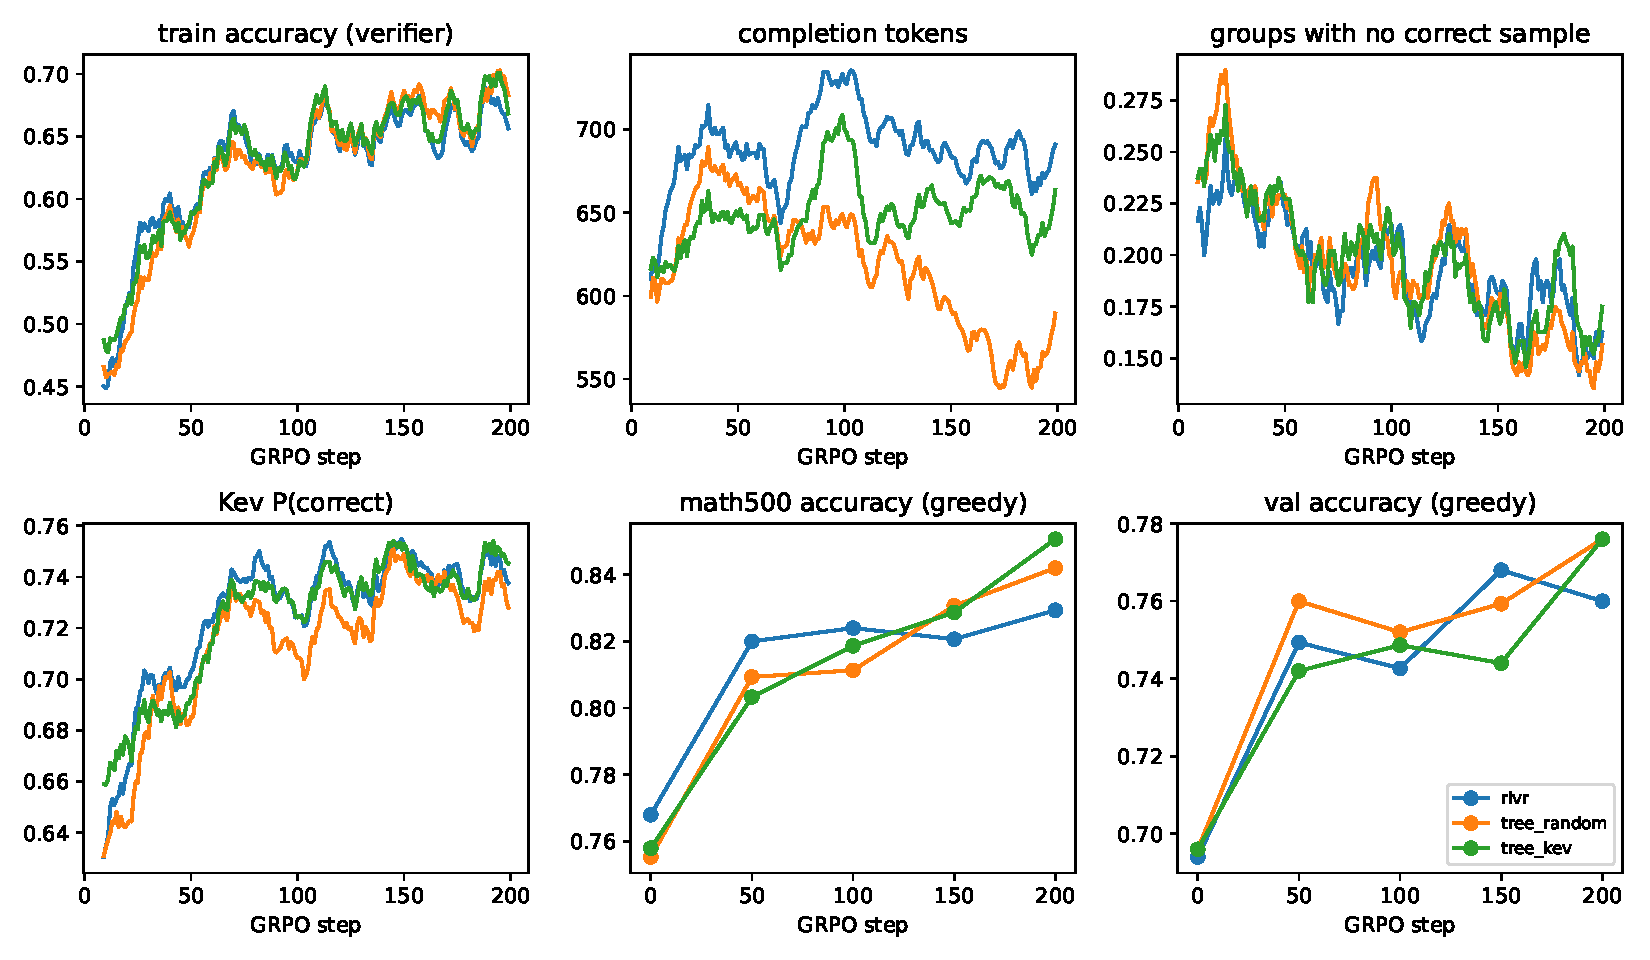
\includegraphics[width=\linewidth]{../../experiments/part3c_tree/results/training_curves.pdf}
\caption{训练曲线（种子均值）：验证器准确率、解答词元数、没有任何正确解答的组的比例，以及 \kev{} 对训练解答给出的 $\pc$（10 步滑动平均）；每 50 步在 MATH-500 和验证集上的贪心准确率。}
\label{fig:tree-curves}
\end{figure}

\paragraph{评估噪声。} 在这一比较的 \NUM{szruns_math500} 个 run 中，基座模型在第 0 步的 MATH-500 准确率介于 \NUM{szmin_math500}\% 和 \NUM{szmax_math500}\% 之间；一个 run 在第 150 步和第 200 步两次评估之间的准确率平均变化 \NUM{lecabs_math500} 个百分点。每个 run 的最终权重都在 MATH-500 上以贪心解码评估了两次：一次是第 200 步的定期评估，一次是最终评估。两次结果平均相差 \NUM{rptabs_math500} 个百分点，最多相差 \NUM{rptmax_math500}（\NUM{rptruns_math500} 个 run）。两次单独评估之间一个百分点左右的差异，在评估本身的噪声之内。

% 第三部分 C：讨论（由 main_zh.tex 引入）。

\section{讨论}\label{sec:discussion}

\paragraph{在一道题内部，评判模型几乎看不出一个解答会走向哪里。} 离线时，\kev{} 的 \emph{on track} 分数区分同一道题 128 词元前缀的正确与错误续写，AUROC 为 \NUM{aucw_128_kevtrack}，不比同样大小的 AR 评判模型（\NUM{aucw_128_artrack}）或策略自身的对数概率（\NUM{aucw_128_logprob}）更好，而后者不需要任何额外代价。合并所有题目时每种信号都更好，因为每种信号都能部分看出题目有多难，而这对在同一道题的前缀中做选择没有帮助。在训练中，面对策略自己的根，这种区分更弱（\NUM{auditotaucw_all_treekev} \ci{\NUM{auditotaucwlo_all_treekev}}{\NUM{auditotaucwhi_all_treekev}}）；保留 \kev{} 在四个根中选出的两个，让正确叶子的比例提高了 \NUM{auditgain_all_treekev} \ci{\NUM{auditgainlo_all_treekev}}{\NUM{auditgainhi_all_treekev}} 个百分点，随机选择为 \NUM{auditgain_all_treerand}，事后最好的两个根为 \NUM{auditbest_all_treekev}。这一收益在训练早期更大（前半段 \NUM{auditgain_firsthalf_treekev} 个百分点，后半段 \NUM{auditgain_secondhalf_treekev}，未给区间）；与此同时，策略的根越来越常导向正确答案，选择的余地也缩小了（事后最好的两个根：\NUM{auditbest_firsthalf_treekev} 和 \NUM{auditbest_secondhalf_treekev} 个百分点）。

\paragraph{根上的小幅收益没有改变策略学到的东西。} 在树形相同时，保留 \kev{} 选出的根而不是随机的根，最终准确率在五个基准上都在按题目重采样的区间内没有变化；GSM8K 上的差值为 \NUM{dvtreerand_treekev_gsm} \ci{\NUM{dvtreerandlo_treekev_gsm}}{\NUM{dvtreerandhi_treekev_gsm}} 个百分点，区间恰好触及零。评判模型选根背后的想法是：它能给 GRPO 更多结果有对有错的组，而只有这样的组才有学习信号。事实并非如此：在最后 20 步中，\texttt{tree\_kev} 下有 \NUM{allwrong_treekev} 的组没有任何正确叶子，\texttt{tree\_random} 下为 \NUM{allwrong_treerand}；全部叶子都正确的组分别为 \NUM{allright_treekev} 和 \NUM{allright_treerand}。这种选择在原理上有代价：被保留的根不再是策略的样本，梯度因而不再是策略梯度的无偏估计。我们没有看到它对准确率的影响。评判模型的选择也没有让策略重复自己：\texttt{tree\_kev} 的一个种子逐渐在第一个答案之后重复解答，但完全没有评判模型的 \texttt{rlvr} 也有一个种子如此，而且 \kev{} 只给解答的前 128 个词元打分，远在答案之前。

\paragraph{树形：种子均值由切换了的种子决定。} 按种子均值，两种树状条件最终都高于扁平采样：MATH-500 上分别高 \NUM{d_treerand_math} 和 \NUM{d_treekev_math} 个百分点，AIME24 上分别高 \NUM{d_treerand_aime24} 和 \NUM{d_treekev_aime24}；但这主要来自改成以纯文本开头写解答的 \NUM{treedraftruns} 个树状 run。它们在 AIME24 上最终为 \NUM{treedraftaime24min}\%--\NUM{treedraftaime24max}\%，其他树状 run 为 \NUM{treeotheraime24min}\%--\NUM{treeotheraime24max}\%，\texttt{rlvr} 为 \NUM{flataime24min}\%--\NUM{flataime24max}\%。同样的切换在整个项目中无论奖励为何都标志着最好的 run（第二部分 \S8.3）。这里树状 run 中有 \NUM{treedraftruns} 个切换，\texttt{rlvr} 的 \NUM{flatruns} 个种子一个也没有。树是否让切换更容易发生，这么少的 run 无法回答；何况这一切换不在我们的计划之中，是在 run 全部结束后才发现的，分类所用的度量也是在读过解答之后定义的。在一棵树里，解答怎样开头由根决定，所以选根同时也是在几种开头之间做选择；随机选根就足以让一个 run 发生切换。树形确定能带来的是词元上的节省：与生成同样长度解答的扁平采样相比，树状 run 每步少生成 \NUM{treegensavemin}--\NUM{treegensavemax} 的词元。

\paragraph{局限。} 只有一种策略规模（4B）、一个对 128 词元的根提出的评判问题（\emph{on track}）、一种树形（四个根，保留两个，每个四个叶子）、以第二部分的学习率训练 200 步，以及每种树状条件 \NUM{seeds_treekev} 个种子（\texttt{rlvr}：\NUM{seeds_rlvr} 个），其中第三个种子是在前两个跑完之后加的。每个提示的根更多时，评判模型可选的余地更大，它犯错的余地也更大。审计每十步才续写全部的根，每个 run 有 20 个审计步；它的区间对这些步重采样，而不对种子重采样。最终准确率的区间对题目重采样，也不对种子重采样。离线研究使用的是基座策略的前缀，而不是训练中策略的前缀。风格的度量是在读过解答之后定义的。我们报告词元数而不是时间：这些 run 与其他实验共用 GPU。

\paragraph{与早期版本的关系。} 本文第 1--3 版报告的剪枝加速、KV 缓存复用率、每节点延迟和定理证明结果（MiniF2F-Lean4、ProofNet）并未经过测量（见文首的说明和 \file{CORRECTION.md}）。这些在本文中都没有测量：我们统计词元而不是时间，也没有做定理证明。凡是我们能检验的，都检验了。v3 的剪枝规则——评判模型的 $p(\text{yes})<0.3$ 时剪掉前缀——用 \emph{on track} 问题时只剪掉 \NUM{thrpruned_128_kevtrack} 的 128 词元前缀，只抓住 \NUM{thrcaught_128_kevtrack} 的死前缀（\S\ref{sec:res-prefix}）。按 \kev{} 选择续写哪些根——这正是那些版本背后的想法——并没有让 GRPO 学得比随机选根更好。


\section*{可复现性}
代码、提示、原始日志（每个 GRPO 步和每次评估）、GRPO run 的每个训练解答，以及前缀研究的解答、前缀、续写和评判分数都在仓库中（\file{experiments/part3c_tree/}）。表格和正文中的每个数字都由 \file{dcjev/llm/prefix_study.py}、\file{dcjev/analysis/part2.py} 和 \file{dcjev/analysis/paper_numbers.py} 从中生成。

\bibliographystyle{plainnat}
\bibliography{../common/refs}
\end{document}
